\documentclass[11pt,letterpaper]{article}
\usepackage[margin=1in,headheight=15pt]{geometry}
\usepackage[T1]{fontenc}
\usepackage[utf8]{inputenc}
\usepackage{lmodern,microtype}
\usepackage{amsmath,amssymb,amsthm,mathtools}
\usepackage{booktabs,longtable,array,enumitem}
\usepackage[dvipsnames]{xcolor}
\usepackage{graphicx,tikz,float}
\usetikzlibrary{arrows.meta,positioning,calc}
\usepackage{fancyhdr}
\usepackage{hyperref}
\usepackage[nameinlink,noabbrev]{cleveref}
\definecolor{Ink}{HTML}{173349}
\definecolor{Accent}{HTML}{236B72}
\hypersetup{colorlinks=true,linkcolor=Ink,citecolor=Accent,urlcolor=Accent,
  pdftitle={Relative Top-Handle Elimination and the Limits of Forest Optimization},
  pdfauthor={ProveIt research continuation},
  pdfsubject={Compressed normal cuts, certified handle cancellation, and unknot recognition}}
\urlstyle{same}
\pagestyle{fancy}
\fancyhf{}
\fancyhead[L]{\small\color{Ink}ProveIt: compressed unknot recognition}
\fancyhead[R]{\small 12 October 2026}
\fancyfoot[C]{\thepage}
\renewcommand{\headrulewidth}{0.3pt}
\setlength{\parskip}{4pt}
\setlength{\parindent}{1.2em}
\setlength{\emergencystretch}{2em}
\setlist{itemsep=3pt,topsep=5pt}
\newtheorem{theorem}{Theorem}[section]
\newtheorem{lemma}[theorem]{Lemma}
\newtheorem{proposition}[theorem]{Proposition}
\newtheorem{corollary}[theorem]{Corollary}
\theoremstyle{definition}
\newtheorem{definition}[theorem]{Definition}
\newtheorem{example}[theorem]{Example}
\newtheorem{question}[theorem]{Research question}
\theoremstyle{remark}
\newtheorem{remark}[theorem]{Remark}
\newcommand{\F}{\mathbb F_2}
\newcommand{\rk}{\operatorname{rank}}
\newcommand{\nul}{\operatorname{null}}
\newcommand{\comp}{\operatorname{comp}}
\newcommand{\bits}{\operatorname{bits}}
\newcommand{\code}[1]{\texttt{\detokenize{#1}}}
\newcommand{\Complete}{\textsf{COMPLETE}}
\newcommand{\Inconclusive}{\textsf{INCONCLUSIVE}}
\newcommand{\core}{K}
\newcommand{\ports}{\mathcal P}
\newcommand{\sourcecommit}{\texttt{8cb7d9d25ac8cb64a9d147304e3441e98e94c7a4}}
\newcommand{\smallpath}[1]{{\small\path{#1}}}

\begin{document}
\hypersetup{pageanchor=false}
\begin{titlepage}
\vspace*{0.10in}
{\large\color{Accent}\sffamily PROVEIT RESEARCH CONTINUATION\par}
\vspace{0.20in}
{\fontsize{27}{31}\selectfont\bfseries\color{Ink}Relative Top-Handle Elimination\par}
\vspace{0.08in}
{\fontsize{21}{25}\selectfont\bfseries\color{Ink}and the Limits of Forest Optimization\par}
\vspace{0.10in}
{\Large in Compressed Unknot Recognition\par}
\vspace{0.22in}
{\normalsize Universal source trees, homological constraints,\par
exceptional-row kernels, and independently replayed certificates\par}
\vspace{0.24in}
Prepared for Vladimir Reshetnikov and the ProveIt project\par
12 October 2026\par
\vspace{0.20in}
\noindent\begin{minipage}{\textwidth}
\small
\textbf{Abstract.}
We remove a concrete unsupported case from ProveIt's compressed normal-cut
pipeline. Every three-handle inherited from an interior source vertex can be
eliminated by source-authenticated two/three-handle cancellations, relative to
the recorded parallelity interfaces. One boundary-rooted tree of the source
one-skeleton specializes to a valid schedule for every admissible normal
surface, including the empty surface and surfaces with arbitrarily large
binary coordinates. The scheduling work is linear in the bounded core size;
the additional trace has $O(t\log(t+2))$ bits.

We then examine whether a better top-handle forest can make the remaining
one/two-handle cancellations succeed. For abstract short occurrence rows this
is a two-graphic-matroid partition problem with an exact rank-deficiency
certificate. A further homological argument substantially narrows its
geometric significance: the boundary-of-boundary identity makes the residual
short-row nullity independent of the forest on the genuine geometric
subclass. We also give an exact contraction kernel for a fixed forest with
arbitrary exceptional rows, isolating the part that requires more than graphic
matroid methods.

The native integration increases independently certified whole-cut censuses
from 85 to 92 on the retained 106-case corpus, preserving all earlier
successes. On a family of genuine subdivided solid tori, the largest measured
case gives a $28.8$-fold scheduling gain and a $1.94$-fold gain when common
source-incidence reconstruction is included. Small cases regress. These are
local advances: a complete quasipolynomial unknot-recognition bound is not
established. The article gives detailed proofs, evidence, integration
contracts, and a research programme aimed at the remaining geometric and
global complexity obligations.
\end{minipage}
\vfill
\noindent\small Based on repository commit \sourcecommit.\par
\noindent\small All performance claims refer to the supplied reproducible
experiments. Mathematical generality, native implementation scope, and
unproved proposals are stated separately.
\end{titlepage}
\hypersetup{pageanchor=true}

\tableofcontents
\newpage
\section{Position of the result}
\label{sec:position}

The immediate outcome is a certified extension of a supplied-normal-cut
primitive. ProveIt's original compressed source construction already retained
the exceptional handles, their attaching charts, and the parallelity
interfaces. Its terminal handlebody consumer refused any core containing a
three-handle. A diagnostic script demonstrated promising deletions, but did
not provide independent source replay. We prove the relative geometric fact
needed for those deletions, reconstruct the missing cap incidences from the
source, and compose the resulting proof with the existing terminal
certificates.

This is consequential because a source interior vertex is an artefact of the
triangulation, not evidence of difficult knot topology. A recognizer should
not lose its compressed terminal operation merely because such a vertex was
introduced. The universal source-tree theorem shows that this obstruction
can be removed uniformly, without searching normal-coordinate supports or
expanding repeated sheets.

\subsection{The quasipolynomial objective and its present status}

For an input knot diagram with $n$ crossings, the intended target is a
deterministic bound of the form
\[
 \exp\bigl((\log(n+2))^{O(1)}\bigr),
\]
with $n^{O(\log n)}$ being the particularly strong form announced in 2021.
The announcement and a proved, implemented end-to-end complexity theorem
must be distinguished. Lackenby's July 2026 preprint presents an algorithm
using incompressible surfaces, boundary patterns, and hierarchies. Its
Section~9 explicitly withholds a running-time estimate for insufficiently
specified steps. Proposition~9.1 bounds the number of steps by
$L(g+1)^L$, in the paper's notation; Proposition~10.2 bounds a refined
partial hierarchy length by $4c_q(\mathcal H)$. A linear hierarchy bound is
not a logarithmic depth bound. Polynomial encoding and verification of an
essential hierarchy in Theorem~14.1 do not give a polynomial procedure for
discovering it~\cite{lackenby2026,oxford2021}.

Our mathematical target is therefore a carefully delimited part of that
programme. A bounded compressed core must support inexpensive geometric
operations with enough source information to justify their use after a cut.
The present top-handle operation meets that requirement for the native
parallelity interfaces. It does not supply arbitrary inherited-pattern
transport, a complete useful-surface search, or a global recurrence bounding
all intermediate representations.

\subsection{What is reused and what is contributed}

Removing three-handles from a compact connected three-manifold with nonempty
boundary is classical. Jackson gives the needed unmarked statement and a
dual-path proof in Lemma~3.2 of~\cite{jackson2023}. The same paper explains
why recovering parallelity-bundle topology is weaker than retaining its
inclusion in the ambient manifold. Our contribution is the source-specific
relative construction, its reusable specialization across all normal cuts,
and its independently verified native implementation. We do not claim a new
general existence theorem for three-handle elimination.

The graph-matroid partition theorem is also classical~\cite{edmondsfulkerson}.
Its application here gives a precise abstract optimization problem and
certificates of optimal residual deficiency. The chain-complex constraint in
\cref{sec:chain}, however, shows why abstract successes cannot automatically
be interpreted as geometric performance gains. This limitation is part of
the research result, not an omitted qualification.

Within ProveIt, the source-parallelity construction, the initial uncut
two/three-handle queue, the stopping-set characterization of positive raw
cancellation, and the saturated-bundle projection are prior work. The ten
incoming packages were audited for these overlaps. In particular,
\emph{Stopping Cores} and \emph{Saturated Bundle Cancellation} already
identify the ten three-handle exclusions and ask for a safe adapter.
\emph{Genus Budgets and Native Interfaces} supplies an initial source
reduction, but not the later normal-cut adapter with its attached
interfaces~\cite{repo,incoming-stopping,incoming-saturated,incoming-genus}.
\Cref{sec:source-audit} records the full targeted overlap audit.

The contributions proved or implemented here are:
\begin{enumerate}
\item A cap-incidence formula for exceptional normal-cut two-handles and a
relative top-handle elimination theorem in the authenticated source charts.
\item A single source tree that specializes to valid traces for every
admissible normal coordinate vector, with coordinate-independent trace size.
\item An exact short-row forest criterion and deficiency formula for the
abstract joint deletion problem, together with an independent prototype.
\item A homological rigidity theorem showing that much of that apparent
forest-choice freedom disappears on genuine geometric inputs.
\item An exact exceptional-row quotient for a fixed forest, which retains
arbitrary long rows and gives a finite pattern kernel.
\item A native version-6 certificate adapter, reproducible coverage gains,
and a controlled local scheduling benchmark with its common costs exposed.
\end{enumerate}

\subsection{Notation and input size}

Let $\mathcal T$ be a finite triangulation of a connected compact orientable
three-manifold $M$ with nonempty boundary. The mathematical source arguments
allow several boundary components. The native validator in this release
accepts the narrower class with exactly one torus boundary. It checks
reciprocal face gluings, orientability, connectedness, sphere or disk vertex
links, circle or interval edge links, and absence of edge reversal. It does
not prove that $M$ came from a knot diagram.

A normal vector $x$ has seven nonnegative integer coordinates in every
tetrahedron, satisfies the matching equations, and uses at most one
quadrilateral type per tetrahedron. Its normal surface is denoted $S_x$.
Zero coordinates and the empty surface are allowed. The metric cut
$M\mathbin{\backslash\!\backslash}S_x$ is the completion after splitting
along the local sheets; this convention also handles one-sided components.
No two-sidedness assumption on $S_x$ is needed for the local results.

\begin{center}
\begin{tabular}{@{}ll@{}}
\toprule
Symbol & Meaning\\
\midrule
$t$ & Number of source tetrahedra\\
$b_x$ & $\sum_{i=1}^{7t}\lceil\log_2(x_i+2)\rceil$, total coordinate bits\\
$K$ & Complementary exceptional handle core of the supplied cut\\
$\ports$ & Complete labelled interface rectangles of the parallelity pieces\\
$q,m$ & Numbers of core three-handles and two-handles\\
$E,C$ & Two-handle row labels and surviving one-handle column labels\\
$G$ & Cap graph, with a formal exterior root $\rho$\\
$H$ & Occurrence graph for rows of capped length at most two\\
$r_G(Y)$ & Graphic rank, $|V(G)|-\comp(G[Y])$\\
\bottomrule
\end{tabular}
\end{center}

The source triangulation takes $O(t\log(t+2))$ bits. The full input size for
the local operation is thus $O(t\log(t+2)+b_x)$, apart from already supplied
source certificates. A word-operation estimate on dense source IDs will
always be distinguished from a bit-complexity bound. In particular, an
$O(t)$ trace is not a claim that reading arbitrarily large coordinates costs
$O(t)$ bit operations.

\section{Relative elimination of source top handles}
\label{sec:relative}

\subsection{The source handle core}

The source-parallelity decomposition divides the metric cut into repeated
product pieces and a bounded exceptional core. Repeated normal disks, face
strips, and edge caps are recorded as affine interval families. Exceptional
tetrahedron chambers give zero-handles; exceptional paired-face regions give
one-handles; extreme gaps of interior source edges give two-handles; and
interior source vertices give three-handles. All attaching records retain
source tetrahedron, face, edge, and rank flags.

For the current constructor the verified inventory bounds are
\begin{equation}
 h_0\leq 6t,\qquad h_1\leq 8t,\qquad
 m=h_2\leq 12t,\qquad q=h_3\leq 4t,\qquad
 |\ports|\leq 66t.
 \label{eq:core-bounds}
\end{equation}
These bounds concern explicit exceptional objects; the represented
parallelity pieces can have much larger multiplicity and topology. Their
complete interfaces, not merely their homeomorphism types, are part of the
source packet~\cite{repo}.

Choose the canonical orientation of each global source edge $e$. Its two
oriented endpoint occurrences are $a_e,b_e$, even if they represent the same
global vertex. Let $w_e=|S_x\cap e|$. The $w_e$ intersection points divide
$e$ into gaps labelled $0,1,\ldots,w_e$. An interior source edge contributes
one exceptional two-handle if $w_e=0$ and two if $w_e>0$. Interior gaps
$1,\ldots,w_e-1$ belong to the selected product region.

For a source vertex $v$, put $\iota(v)=v$ when $v$ is interior and
$\iota(v)=\rho$ when it lies on the original boundary. The symbol $\rho$
also denotes an end on the new normal-cut boundary.

\begin{lemma}[Exact cap incidences]
\label{lem:caps}
For an interior source edge $e$, the two belt-disk end occurrences of its
exceptional two-handles are
\[
\begin{array}{c|c|c}
 \text{condition}&\text{gap rank}&\text{cap endpoints}\\\hline
 w_e=0&0&(\iota(a_e),\iota(b_e))\\
 w_e>0&0&(\iota(a_e),\rho)\\
 w_e>0&w_e&(\rho,\iota(b_e)).
\end{array}
\]
The two occurrences are retained with multiplicity. In particular, a
zero-weight loop at an interior vertex has two contacts with its
three-handle.
\end{lemma}

\begin{proof}
Before taking any quotient of source flags, take a small product
neighbourhood of each open edge gap. Transversely it is a disk; longitudinally
it is the indicated subinterval of the oriented edge. The transverse disk
times this interval is its dual two-handle. An endpoint at a source vertex
meets the vertex neighbourhood, which is a three-handle exactly when the
vertex link is a sphere. A boundary vertex has a disk link and contributes
an exterior end instead.

An endpoint at an intersection with a normal disk lies on a boundary sheet
of the metric cut. Thus a zero-weight edge keeps both source-vertex ends,
whereas each extreme gap of a positive-weight edge has one source-vertex end
and one cut-boundary end. The intervening gaps have two normal-sheet ends
and occur in the product families. The source edge-link and orientation
checks ensure that this description descends through all face identifications.
A global equality $a_e=b_e$ does not identify the two oriented end flags.
The argument is local to the split sheets, so a one-sided global normal
component causes no exception.
\end{proof}

\begin{figure}[htbp]
\centering
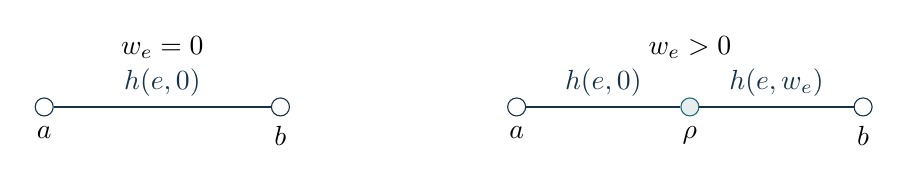
\begin{tikzpicture}[x=1cm,y=1cm,>=Stealth,
  vertex/.style={circle,draw=Ink,fill=white,inner sep=2.3pt},
  root/.style={circle,draw=Accent,fill=Accent!12,inner sep=2.3pt}]
 \node[vertex,label=below:$a$] (a) at (0,0) {};
 \node[vertex,label=below:$b$] (b) at (3,0) {};
 \draw[thick,Ink] (a)--node[above]{$h(e,0)$}(b);
 \node at (1.5,0.75) {$w_e=0$};
 \node[vertex,label=below:$a$] (c) at (6,0) {};
 \node[root,label=below:$\rho$] (r) at (8.2,0) {};
 \node[vertex,label=below:$b$] (d) at (10.4,0) {};
 \draw[thick,Ink] (c)--node[above]{$h(e,0)$}(r);
 \draw[thick,Ink] (r)--node[above]{$h(e,w_e)$}(d);
 \node at (8.2,0.75) {$w_e>0$};
\end{tikzpicture}
\caption{The cap graph records the extreme gaps. The common drawing of
 $\rho$ is a scheduling convention; distinct boundary pieces are never
 identified in the manifold. Boundary source vertices also map to $\rho$.}
\label{fig:caps}
\end{figure}

\subsection{The relative geometric hypothesis}

A graph trace alone cannot justify a marked three-manifold operation. The
entire protected interface must avoid the support of the cancellation.
Even the assertion that ports lie on zero- and one-handles is insufficient:
a three-handle attaching sphere can meet patches of those lower handles.
The native argument uses the actual rank charts.

\begin{lemma}[Separation in the source rank charts]
\label{lem:separation}
In the source-parallelity decomposition, the labelled interface rectangles
$\ports$, with compatible corner collars, can be realized disjointly from
the interiors and attaching regions of the exceptional two/three-handle
cancellation supports. This realization respects all source identifications
and the specified port charts.
\end{lemma}

\begin{proof}
Work first in the split tetrahedra, with their source flags kept distinct.
Choose mutually compatible small regular neighbourhoods of vertex sectors,
edge-gap sectors, and paired-face sectors. The normal disks bound the split
regions and separate their successive gap interiors. This is a finite PL
construction for each supplied $x$; it is used to prove the interpretation
of the compressed families, not to enumerate them.

A prism family has ranks $1\leq r<n$ between successive parallel disks of
one type. A face-strip family has ranks $1\leq r<a$ between successive
parallel normal arcs at its corner. An edge-cap family has ranks
$1\leq r<w_e$. These are strict interior ranks. The vertex sectors lie at
the source ends of the ordered gaps. The exceptional two-handles occupy
rank $0$, and also rank $w_e$ when $w_e>0$. Thus a selected product block
does not occupy a source vertex sector or an exceptional end-gap sector.
When an extreme gap and an interior product gap abut the same normal disk
before cutting, their closures lie on different local boundary copies in
the metric cut. This local separation also applies to a one-sided surface.

The core-facing free sides of a face-strip or edge-cap block are the
recorded port rectangles. Their source chamber and face flags are retained,
including for self-paired tetrahedra. If closures meet a lower-dimensional
corner during the initial subdivision, choose product collars on the two
flagged sides and round inside their respective sectors. Strict interior
rank places the port on the side separated from the end-gap/vertex
neighbourhood; no passage through a normal disk is required. Since the
paired rank maps agree along a source face, the collar choices can be made
equivariantly under each pairing. Edge and vertex links being a circle,
interval, sphere, or disk give precisely the local PL neighbourhoods needed
for simultaneous rounding.

After this compatible rounding the full port rectangles and their collars
miss the vertex balls and the selected exceptional two-handles, including
their lateral attaching annuli and their incident vertex-ball patches.
The proof uses the full source product blocks. It would not follow from a
list of port owner dimensions or a matrix of signed exponents.
\end{proof}

\begin{remark}
The protected set in \cref{lem:separation} is the native parallelity
interface. A future inherited boundary-pattern curve can cross a vertex
patch or an extreme-gap support even when it is carried by a zero/one
skeleton. Such a curve requires a separate avoidance or transport proof.
This article does not silently enlarge $\ports$ to an arbitrary pattern.
\end{remark}

\subsection{One cancellation and a complete rooted schedule}

\begin{lemma}[Relative single-contact cancellation]
\label{lem:relative-move}
Let $h$ be an exceptional two-handle with exactly one contact, counted with
multiplicity, with the currently remaining three-handles. Let that contact
be with $D$. Assume that the other cap of $h$ is on the current exterior
boundary and that the marked interface misses the cancellation support.
Removing $h$ and $D$ gives a homeomorphic manifold relative to that
interface. Each surviving two-handle keeps its original attaching cycle to
the zero/one-handle union. Its cap contacts with $D$ become exterior contacts.
\end{lemma}

\begin{proof}
This is a two/three-handle cancellation with geometric incidence one. In
the source handle charts, $h$ and $D$ are balls glued along their unique
common cap disk. Their union is a ball. Its attachment to the remaining
handles is a disk: the complementary disk in the attaching sphere of $D$
is extended by the lateral attaching annulus of $h$. The other cap is
exterior. Removing a ball attached along a boundary disk preserves the
homeomorphism type by adjusting a collar of that disk.

The collar can be chosen away from the protected interface. This gives a
homeomorphism fixed on the interface and its specified charts. It does not
assert that every point of every undeleted lower handle is fixed: the
attaching-disk collar must move. The reduced presentation itself consists
of the undeleted handles, whose mutual attaching records remain unchanged.
In particular, the other two-handle attaching cycles are literally the
same records. Only their upper cap status changes when $D$ is erased.
\end{proof}

Define the cap multigraph $G_x$ on the $q$ interior vertex three-handles and
the formal root $\rho$. Each exceptional two-handle is an edge with the
endpoint occurrences in \cref{lem:caps}. An exterior--exterior handle is a
loop at $\rho$. A loop at an interior vertex is also retained as a loop,
with two incidences.

\begin{lemma}[Rooted deletion criterion]
\label{lem:rooted}
For any such cap graph, all three-handles can be deleted by single-contact
steps if and only if every graph vertex reaches $\rho$. The edge sets of
complete schedules are exactly the spanning trees of $G_x$.
\end{lemma}

\begin{proof}
Given a spanning tree rooted at $\rho$, delete each vertex after its parent,
using the edge to that parent. At that instant the edge has exactly one live
endpoint. Conversely, orient each chosen edge from the vertex it deletes
toward its other end. That end is $\rho$ or a previously deleted vertex.
Following the chosen edges therefore reaches $\rho$ and never forms a
cycle. Exactly $q$ edges are selected on $q+1$ vertices, so they form a
spanning tree. A component not meeting $\rho$ cannot supply its first legal
step. A loop never has exactly one live endpoint.
\end{proof}

\begin{theorem}[Source-relative top-handle elimination]
\label{thm:top}
For every admissible normal vector in the stated source setting, all $q$
source three-handles can be removed by exactly $q$ exceptional two/three
cancellations. The resulting core $K'$ has no three-handles and satisfies
\[
 (K,\ports)\cong(K',\ports).
\]
All labelled port rectangles and charts, all zero/one-handle IDs, and all
surviving two-handle attaching cycles can be retained. Reattaching the same
parallelity pieces along the same interfaces gives a homeomorphic whole
cut.
\end{theorem}

\begin{proof}
Consider a component $U$ of the graph of zero-weight source edges on the
interior vertices. A positive-weight edge incident to $U$ gives an exterior
contact by \cref{lem:caps}. A zero-weight edge from $U$ to a boundary vertex
does the same. If neither occurred, every source edge incident to $U$ would
have weight zero and both ends in $U$. This would isolate $U$ in the source
one-skeleton, contrary to connectedness of that skeleton and nonemptiness
of the source boundary. Hence every such component reaches an exterior
contact, and $G_x$ is rooted-connected.

Use \cref{lem:rooted} for the schedule, \cref{lem:separation} for its protected
interface, and \cref{lem:relative-move} for each step. Induction gives the
relative homeomorphism. Boundary components represented by the same formal
root are never glued together: every actual cancellation has only one live
three-handle end. Finally, a homeomorphism fixed on the entire gluing
interface extends by the identity over every reattached parallelity piece.
\end{proof}

Deleting equal numbers of two- and three-handles preserves Euler
characteristic. Surviving two-handle IDs may be densely renumbered for the
old terminal consumer after source replay, but a certificate must record
the original IDs used by the trace. This distinction prevents an accidental
reassignment of attaching cycles when rows are removed.

\section{One source tree for every normal cut}
\label{sec:templates}

The cap graph changes when a source edge weight becomes positive. It would
be wasteful to regard each zero/nonzero support as an unrelated scheduling
problem. The source one-skeleton already supplies one schedule template for
all of them.

\begin{definition}[Boundary-rooted source forest]
Choose a forest $T_0$ in the source vertex graph such that every interior
vertex has a unique parent edge and every component has one source boundary
vertex as its root. There is no parent edge for a boundary vertex. Record the
interior vertices in a parent-before-child order. Such a forest is produced
by a multi-source breadth-first search starting at all boundary vertices.
\end{definition}

The term forest refers to the actual source vertices. Contracting all
boundary roots to one formal vertex makes its interior portion a rooted
tree for the scheduling argument. This is still only graph bookkeeping.

\begin{theorem}[Universal source-tree specialization]
\label{thm:template}
Fix $T_0$ independently of normal coordinates. For every admissible $x$,
process its interior vertices in the recorded order. For a vertex $v$ with
parent edge $e$, choose
\begin{enumerate}
\item the unique exceptional gap of $e$, when $w_e=0$;
\item the extreme gap of $e$ adjacent to $v$, when $w_e>0$.
\end{enumerate}
Cancel that two-handle with the three-handle of $v$. This is a complete
valid trace for the relative operation of \cref{thm:top}. The same source
template works for all admissible coordinate supports and all scales.
\end{theorem}

\begin{proof}
An edge incident to an interior vertex is not a boundary edge, so the
required exceptional gap exists. If its weight is zero, its other endpoint
is the parent, which is a boundary vertex or has already been removed. It
therefore has exactly one live three-handle contact, namely $v$. If its
weight is positive, the child-adjacent extreme gap has its other endpoint on
the new cut boundary; it is immediately eligible, regardless of the
parent's status.

Distinct vertices use distinct parent edges of the source forest. Two
different choices can consequently never request the same exceptional
two-handle, including after a support change replaces one zero gap by two
extreme gaps. A parent edge cannot be an interior loop. Every interior
vertex is processed once, and \cref{lem:relative-move} applies at every
step. The construction makes no assumption on coordinate size and includes
$x=0$.
\end{proof}

\begin{corollary}[Support and scale invariance]
\label{cor:support}
The cap graph, considered with oriented extreme-gap labels, depends on $x$
only through the predicates $w_e=0$. Positive scaling $x\mapsto kx$ leaves
the source-tree choices and the corresponding dense two-handle IDs
unchanged. A specialized trace has the same number of moves and source-ID
bits at every positive scale.
\end{corollary}

\begin{proof}
The cap formula only distinguishes zero from positive weight. In the latter
case the numerical label $w_e$ changes but the order of the two extreme
gaps does not. Source vertices, source edge order, and the parent forest
are fixed. The trace records source handle IDs, while its input fingerprint
has fixed encoded length.
\end{proof}

The corollary concerns the added top trace. The complete source certificate
still contains exact coordinates and affine endpoints and can grow with
$b_x$. It would be incorrect to infer constant total proof size from constant
top-trace size.

\subsection{A linear queue and an independent trace checker}

The default implementation uses a queue rather than requiring the reusable
template. Initialize every edge with one live endpoint. When a vertex is
deleted, revisit its incident edges and enqueue newly eligible ones.
Duplicate queue entries are harmless: a popped edge is checked against the
current live sets before use. Each interior loop is stored once in the
vertex adjacency list but retains both endpoint occurrences in the edge
record.

\begin{proposition}[Local cost and trace size]
\label{prop:cost}
Given an authenticated dense-ID cap packet with $m$ edges and $q$ interior
vertices, a complete rooted schedule and the surviving edge list can be
produced in $O(m+q)$ word operations and $O(m+q)$ space. The supplied trace
can be checked in the same structural bound. For the source cores in
\eqref{eq:core-bounds}, the additional proof takes
$O(t\log(t+2))$ bits. Source validation, coordinate reading, rank address
reconstruction, and fingerprinting remain polynomial in
$t\log(t+2)+b_x$.
\end{proposition}

\begin{proof}
The initialization and final dense-ID survivor scan visit each edge once.
There are at most $2m$ vertex--edge incidences. Each is revisited only when
its vertex is deleted. Each visit performs constant work on an edge's two
endpoint occurrences and can enqueue it at most once. The initial queue
also has at most $m$ entries. Thus all queue pops and endpoint checks have
linear total count. A checker reads each of the $q$ pairs, rejects reuse,
and tests its at most two live contacts. It finally compares the exact
survivor list.

All original handle IDs are $O(t)$, so the $q$ pairs and at most $m$
survivors use $O(t\log(t+2))$ bits. The template also consists of $O(t)$
vertex, parent, and source-edge labels of this length. Reconstructing the
source data requires a polynomial number of combinatorial operations and
arithmetic on the input integers. No loop ranges over the numerical normal
weight, and the fingerprint uses hexadecimal coordinate encodings rather
than decimal conversions with implementation-specific digit limits.
\end{proof}

The public template functions validate their source arguments rather than
assuming a previously trusted cache. Thus their current complete-call cost
includes source validation even when the combinatorial template is reused.
A future authenticated session object could remove duplicate validation
work while preserving the source binding. Such caching is a separate
implementation improvement, not part of the linear queue claim.

\subsection{How the source orientation is authenticated}

A triangulation edge can appear in many local tetrahedra, and its two global
endpoint vertices can coincide. The canonical orientation is determined by
the signed source edge union, not by sorting vertex labels. The producer
uses the union-find root's own oriented local representative. The verifier
uses a different reconstruction: it scans \emph{every} local occurrence,
reverses its endpoint pair according to the recorded orientation parity,
and demands agreement.

This matters in practice. The general source validator keeps a convenient
last-seen endpoint pair that is sufficient for link counting but need not
be in the canonical orientation. Using that pair to decide which extreme
gap has rank zero can reverse the cap formula. The new proof checker does
not trust that shortcut. It reconstructs the complete expected exceptional
rank inventory before interpreting any move.

\subsection{The exact scope of uniformity}

The template is universal for one fixed source triangulation. A subsequent
hierarchy state may have a different triangulation or a differently
represented marked handle structure. The theorem does not identify those
states, transport their patterns, or establish a bounded number of source
rebuilds. Its useful implication is more local: within a fixed source,
top-handle elimination introduces no branch over normal supports and no
normal-weight-dependent number of moves.

\section{Joint forest selection in the abstract occurrence model}
\label{sec:joint}

The top-handle theorem allows many possible deletion trees. The rows left
behind can differ, so it is natural to ask whether a tree can be chosen to
make the subsequent one/two-handle cancellation easy. This section solves
an exact abstract version of that problem. The geometric constraint in the
next section is indispensable when interpreting the answer.

\subsection{Raw occurrences, saturation, and peeling}

Fix the primal forest used to cancel the zero/one-handle forest. The
remaining one-handles have labels $C$, and the original two-handles have
labels $E$. Let
\[
 a_{ec}\in\mathbb Z_{\geq0}
\]
be the actual unsigned number of passages of the attaching curve of $e$
through the cocore of $c$. These are geometric occurrences, not freely
reduced words or signed exponent sums. For the native core they are obtained
by counting the dimension-one flags of the source attaching cycles after
omitting the primal forest columns.

\begin{definition}[Unit-column peeling]
For a live row set $R\subseteq E$, a pivot $(e,c)$ is a unit-column pivot
if $e\in R$ and
\[
 \sum_{f\in R} a_{fc}=a_{ec}=1.
\]
Peeling this pivot deletes row $e$. The other rows remain unchanged, and
column $c$ becomes zero. A row set is peelable if all its rows can be
deleted this way.
\end{definition}

Put $b_{ec}=\min(2,a_{ec})$. Every unit-column predicate on every row
subset is unchanged by this entrywise saturation: a nonnegative sum is one
exactly when it consists of one unit contribution and otherwise zeros. We
therefore use $b$ for peeling, retaining $a$ when integral or mod-two chain
information is needed.

A nonempty row set $Z$ is a \emph{stopping set} if each of its column sums
is zero or at least two. Its first row can never be peeled, even with other
rows present. Conversely, a stalled peeling process leaves a stopping set.
Unions of stopping sets are stopping sets, so their largest union is the
canonical residual. These statements and the equivalence with complete
positive raw cancellation are prior results in the incoming
\emph{Stopping Cores} report~\cite{incoming-stopping}. The present paper
uses them within that exact positive model. Allowing geometric slides with
intersection cancellation or changing the cocore system is a different
problem.

No arbitrary columns may be discarded. If private bundle columns are
omitted, an independent geometric projection theorem must already justify
the omission, as in the saturated-bundle work. The combinatorial theorems
below can be used on any designated matrix, but a manifold interpretation
requires an authenticated producer for precisely that matrix.

\subsection{Short rows form a graph}

Call $e$ short if $\sum_c b_{ec}\leq2$. Introduce an auxiliary ground
vertex $\omega$, distinct from the cap-graph root $\rho$. The occurrence
multigraph $H$ has vertices $C\cup\{\omega\}$ and one labelled edge for
every short row:
\begin{center}
\begin{tabular}{@{}ll@{}}
\toprule
Nonzero entries of the short row & Its edge in $H$\\
\midrule
One unit at $c$ & $c\omega$\\
Two units at distinct $c,d$ & $cd$\\
One entry at least two at $c$ & A loop at $c$\\
No entries & A loop at $\omega$\\
\bottomrule
\end{tabular}
\end{center}
The last case is necessary: an empty two-handle row cannot be deleted by a
one/two-handle pivot. Parallel edges and loops are genuine cycles.

\begin{lemma}[Graphic peeling criterion]
\label{lem:graphic}
A set of short rows $R$ is completely peelable if and only if $H[R]$ is a
forest.
\end{lemma}

\begin{proof}
At a nonground vertex, the graph degree equals the saturated column sum,
with a loop counted twice. A nonempty forest component has at least two
leaves. At most one leaf is $\omega$, so there is a nonground degree-one
vertex and therefore a legal unit-column pivot. Removing its edge preserves
the forest, and induction peels every row.

Conversely, the edges of any cycle form a stopping set. At every nonground
vertex their degree is zero or at least two. This includes an interior
loop, a loop at $\omega$, and a two-edge cycle of parallel edges. None of
these edge sets can have a first peeled row.
\end{proof}

\subsection{The two-forest criterion}

First suppose every row is short, and let $G$ be the connected cap graph on
the same edge label set $E$. By \cref{lem:rooted}, a complete top schedule
deletes a spanning tree $F$ of $G$. Its complement must be an $H$-forest if
the residual rows are to peel.

\begin{theorem}[Abstract joint forest criterion]
\label{thm:joint}
For connected $G$ and short-row graph $H$, the following are equivalent:
\begin{enumerate}
\item There is a spanning tree $F$ of $G$ such that $H[E\setminus F]$ is
a forest.
\item $E$ is a disjoint union of a $G$-forest and an $H$-forest.
\item For every $Y\subseteq E$,
\begin{equation}
 |Y|\leq r_G(Y)+r_H(Y).
 \label{eq:rank-test}
\end{equation}
\end{enumerate}
A deterministic polynomial-time procedure finds the two schedules or a
subset violating \eqref{eq:rank-test}.
\end{theorem}

\begin{proof}
The first condition immediately gives the second. Given a partition into
forests $I_G,I_H$, extend $I_G$ to a spanning tree by moving edges from
$I_H$. If $I_G$ does not yet span, connectedness of $G$ supplies an edge of
$I_H$ between different $I_G$ components. Adding it preserves the
$G$-forest; removing it preserves the $H$-forest. Repeat. This proves the
first condition and gives the two schedules by \cref{lem:rooted,lem:graphic}.

Intersecting a forest partition with $Y$ proves necessity of
\eqref{eq:rank-test}. Sufficiency is the two-matroid partition theorem of
Edmonds--Fulkerson~\cite[Theorem 1c]{edmondsfulkerson}. For completeness,
the explicit augmenting proof and its witness are given below.
\end{proof}

Now let
\[
 D=\{e:\textstyle\sum_c b_{ec}>2\},\qquad E_0=E\setminus D.
\]
Consider the restricted strategy that requires all rows of $D$ to be
deleted by the top-handle forest. This is a restriction of the strategy,
not a necessary condition for raw cancellation. The single row $(1,1,1)$
is already peelable.

\begin{corollary}[Forced long rows]
\label{cor:forced}
The restricted strategy is possible exactly when $G$ is connected,
$G[D]$ is a forest, and for all $Y\subseteq E_0$,
\begin{equation}
 |Y|\leq r_G(Y\cup D)-|D|+r_H(Y).
 \label{eq:forced-rank}
\end{equation}
Here $H$ is the short-row graph on $E_0$. When $D$ is independent, the first
two terms on the right are $r_{G/D}(Y)$.
\end{corollary}

\begin{proof}
A spanning tree can contain $D$ only when $D$ is a forest. Contracting this
forest identifies spanning trees containing $D$ with spanning trees of
$G/D$. Graphic matroid contraction has rank
$r_{G/D}(Y)=r_G(Y\cup D)-r_G(D)$, and $r_G(D)=|D|$.
Apply \cref{thm:joint}. Contraction can create loops and parallel edges;
they remain in the instance.
\end{proof}

\subsection{A constructive proof with a failure certificate}
\label{sec:augment}

Write $G'=G/D$, with $D=\varnothing$ in the unforced case. Maintain
disjoint sets $I_0,I_1\subseteq E_0$, independent in $G'$ and $H$,
respectively. All other edges are unassigned. An edge $e\notin I_i$ is an
$i$-sink if adding it to $I_i$ preserves a forest. Otherwise its endpoints
are joined by the unique path in the forest $I_i$. Draw an exchange arc
$e\to f$ for each path edge $f$. For a loop this path has no edges and
there is no exchange arc.

Run breadth-first search in this exchange digraph, starting at every
unassigned edge. If a shortest source-to-sink path
$e_0,e_1,\ldots,e_\ell$ is found, put its terminal edge into its sink
forest. For every $j<\ell$, assign $e_j$ to the old forest of
$e_{j+1}$. The number of assigned edges increases by one.

Here is an explicit independence argument. Represent graph edges by their
endpoint incidence vectors over $\F$. Forest edge vectors are independent.
For an incoming edge $e_j$, its expansion in its target forest has
coefficient one on $e_{j+1}$. It has coefficient zero on every later
removed edge $e_{k+1}$ of that same forest, $k>j$: otherwise there would be
an exchange arc skipping part of the shortest path. The matrix of these
coefficients on the removed edges is triangular with diagonal one.
Replacing the removed forest edges by the corresponding incoming edges
therefore preserves the old span and independence. No earlier path vertex
was a sink, since that would give a shorter path. The terminal edge lies
outside the old span of its sink forest and increases its rank by one.
This proves the augmentation rule.

If no sink is reachable, let $Y$ be the reached edge set and $U$ the
unassigned set. Then $U\subseteq Y$. Every fundamental path reached in
either forest lies entirely in $Y$. Consequently
\[
 r_i(Y)=|I_i\cap Y|\quad(i=0,1),\qquad
 |Y|-r_0(Y)-r_1(Y)=|U|.
\]
When $U\ne\varnothing$ this is a violated rank inequality. It also proves
optimality of the current partial partition: any two-forest union has size
at most
\[
 |E_0\setminus Y|+r_0(Y)+r_1(Y)=|E_0|-|U|,
\]
and the current partition attains this value. When $U=\varnothing$, all
edges are assigned and the desired full partition has been found.

For $m_0=|E_0|$ and $v=|V(G')|+|V(H)|$, the simple implementation has at
most $m_0$ augmentations. Each search visits at most $m_0$ edge labels and
uses ordinary forest-path traversals. Its conservative structural bound is
\[
 O\bigl(m_0^2(v+m_0)+m_0^3\log(m_0+2)\bigr).
\]
Integer parsing, label comparisons, and source authentication are additional
polynomial bit costs. Large occurrence values are compared with two, never
expanded into repeated crossings by this planner.

\subsection{An exact residual-deficiency theorem}

When the restricted strategy cannot finish, its failure need not be reported
only as a boolean. Assume $G$ is connected and $D$ is a forest. Define
\begin{equation}
 d=\max_{Y\subseteq E_0}
 \bigl(|Y|-r_{G/D}(Y)-r_H(Y)\bigr).
 \label{eq:deficiency}
\end{equation}
The empty set makes $d\geq0$.

\begin{theorem}[Optimal residual nullity]
\label{thm:deficiency}
The deficiency satisfies
\begin{equation}
 d=\min_{\substack{F\text{ spanning tree of }G\\D\subseteq F}}
 \bigl(|E\setminus F|-r_H(E\setminus F)\bigr).
 \label{eq:minmax}
\end{equation}
The exchange procedure produces an attaining tree, an occurrence forest in
its residue, and a rank witness certifying the common optimum.
\end{theorem}

\begin{proof}
The augmentation argument proves that the maximum two-forest union in
$E_0$ has size $m_0-d$. For any tree $F\supseteq D$, let $J$ be a maximum
$H$-forest in its residue $R=E\setminus F$. Then $F\setminus D$ and $J$
are a two-forest union, so
\[
 |F\setminus D|+r_H(R)\leq m_0-d.
\]
Since $|F\setminus D|+|R|=m_0$, the residual nullity is at least $d$.

For the reverse inequality, take a maximum partial partition $I_G,I_H$.
Every unassigned edge has endpoints in one $I_G$ component; otherwise it
could be assigned to that forest. Hence $I_G\cup I_H$ spans the connected
graph $G/D$. Extend $I_G$ to a spanning tree $T$ using edges of $I_H$ only.
The unused part $J\subseteq I_H$ remains an $H$-forest. Its complement in
$E_0\setminus T$ consists of exactly the $d$ unassigned edges. Therefore
\[
 |E_0\setminus T|-r_H(E_0\setminus T)
 \leq |E_0\setminus T|-|J|=d.
\]
Lift $T$ through the contracted forest $D$. This attains the lower bound.
\end{proof}

The number $d$ is the minimum number of \emph{additional arbitrary row
deletions} that would make an optimized residue a forest. Such deletions are
not licensed geometric cancellations and are never performed by the
prototype. The certificate measures the exact abstract obstacle; it is not
a proof that the manifold is not a handlebody.

\subsection{Two instructive limitations}

\begin{example}[An abstract exchange gain with no geometric realization]
\label{ex:abstract}
Take two interior cap vertices $u,v$ and three rows:
\[
\begin{array}{c|c|c}
e&\text{cap edge in }G&\text{single-column occurrence row}\\\hline
0&uv&(1)\\
1&v\rho&(0)\\
2&u\rho&(2).
\end{array}
\]
Deleting edges $0,1$ leaves the unpeelable row $(2)$; deleting $1,2$
leaves $(1)$ and succeeds. This is a genuine test of the abstract exchange
algorithm. It is not an example of a three-manifold improvement. Over
$\F$, its occurrence boundary and cap incidence have nonzero product:
each interior vertex column sees the unit contribution from row $0$.
It violates $\partial_2\partial_3=0$. \Cref{sec:chain} explains the
consequence of imposing that identity.
\end{example}

\begin{proposition}[General peelability is not a matroid]
\label{prop:not-matroid}
The peelable row subsets of an arbitrary nonnegative occurrence matrix
need not satisfy the matroid augmentation axiom.
\end{proposition}

\begin{proof}
Use the four binary rows
\[
 a=(0,0,1),\quad b=(0,1,1),\quad
 c=(1,1,0),\quad f=(1,1,1).
\]
Both $I=\{c,f\}$ and $J=\{a,b,c\}$ peel: in $I$ first use the third
column of $f$; in $J$ first use the first column of $c$, then the second
of $b$, then the third of $a$. Yet $|J|>|I|$ and neither $I\cup\{a\}$
nor $I\cup\{b\}$ peels. Every nonzero column sum in either enlarged set
is at least two. Thus augmentation fails.
\end{proof}

This counterexample does not prove hardness of the general geometric
problem. It identifies the precise reason that the short-row matroid
argument cannot simply be extended to arbitrary long rows.

\section{The chain constraint: when forest optimization disappears}
\label{sec:chain}

The two-graph model has an additional constraint on native geometric inputs.
Its cap incidences and raw attaching counts are parts of the same cellular
chain complex. This constraint makes a substantial part of the apparent
forest-choice problem collapse to one tree extension. It also provides a
necessary realizability check for proposed abstract examples.

\subsection{Raw parity and complementary tree coordinates}

Fix an authenticated core $K$ and a geometric forest contraction among its
zero- and one-handles. Let $E$ index its $m$ two-handles, let $C$ index the
remaining one-handles, and let $q$ be the number of three-handles. Write
$a_{ec}$ for the \emph{uncapped} geometric occurrence count of one-handle
$c$ in the attaching cycle of two-handle $e$. Define
\[
 A=(a_{ec}\bmod 2)\in\F^{E\times C},\qquad
 B\in\F^{E\times\{1,\ldots,q\}},
\]
where $B_{ev}$ counts the cap occurrences of $e$ at three-handle $v$ modulo
two. Both ends of a loop are counted. Orientations disappear over $\F$,
but geometric occurrences must be counted before reduction modulo two.

The handle chain complex gives
\begin{equation}
 \partial_2=A^{\mathsf T},\qquad
 \partial_3=B,\qquad A^{\mathsf T}B=0.
 \label{eq:boundary-boundary}
\end{equation}
The matrix $B^{\mathsf T}$ is the reduced incidence matrix of the cap graph
$G$, with the formal exterior root omitted. By \cref{thm:top}, $G$ is
connected in the native source setting. Hence $\rk B=q$, and
\begin{equation}
 \beta_2(K;\F):=\dim_{\F}H_2(K;\F)=m-\rk A-q.
 \label{eq:chain-beta}
\end{equation}
Several core components cause no problem when each reaches an exterior
end: the common graph root is formal and the three-handle columns remain
independent. Closed components with nonzero $H_3$ require a different rank
statement.

Suppose first that every \emph{raw} row has length at most two. Construct
the occurrence graph $H$ as in \cref{sec:joint}: singleton rows join their
column to a ground vertex, two distinct occurrences join their columns,
and double occurrences or empty rows are loops. Then $A^{\mathsf T}$ is
exactly a reduced incidence representation of $H$. Write $r_H(S)$ for its
graphic rank on edge set $S$, and $\nu_H(S)=|S|-r_H(S)$ for its cycle
nullity.

\begin{theorem}[Geometric short-row invariance]
\label{thm:chain-invariance}
If $\sum_c a_{ec}\leq2$ for every $e\in E$, then every spanning tree $F$ of
the cap graph satisfies
\begin{equation}
 r_H(E\setminus F)=r_H(E),\qquad
 \nu_H(E\setminus F)=\beta_2(K;\F).
 \label{eq:tree-invariance}
\end{equation}
Consequently, one such residue admits complete unit-column peeling if and
only if every such residue does. Changing the top-handle tree cannot
improve its occurrence-graph nullity.
\end{theorem}

\begin{proof}
Transposing \cref{eq:boundary-boundary} gives
\[
 \operatorname{col}(A)\subseteq\ker(B^{\mathsf T}),
\]
the cycle space of $G$. Projection onto the coordinates $E\setminus F$ is
injective on this cycle space: a vector in its kernel would be a cycle
supported entirely on a forest, and therefore zero. The same projection
is injective on $\operatorname{col}(A)$, so $\rk A_{E\setminus F}=\rk A$.
These ranks are respectively $r_H(E\setminus F)$ and $r_H(E)$.

Every cap spanning tree has $q$ edges. Substitution in
\cref{eq:chain-beta} proves the nullity identity. Finally, the short-row
peeling criterion of \cref{sec:joint} identifies complete peeling with
zero occurrence-graph nullity.
\end{proof}

This is a restriction on the optimization problem, rather than a defect
in the abstract matroid theorem. In compatible geometric inputs, the row
space representing $H$ lies in the cycle space of $G$. The two graphs
cannot be varied independently.

\subsection{Mandatory rows and the homological criterion}

Capping counts at two preserves singleton predicates but can change
parity. For example, a raw row $(3)$ has binary row $(1)$, whereas its
capped row $(2)$ represents a loop and hence a zero incidence column.
With no three-handles, this example has $m-\rk A-q=0$ but occurrence-graph
nullity one. Thus \cref{thm:chain-invariance} cannot simply be applied to
arbitrary capped short rows.

There is an exact repair for the restricted strategy. Put
\begin{align}
 D_{\mathrm{long}}&=\bigl\{e:\sum_c\min(2,a_{ec})>2\bigr\},\notag\\
 D_{\mathrm{loop}}&=\{e:a_e=0\text{ or }a_e=k\mathbf e_c
                         \text{ for some }k\geq2\},\notag\\
 \overline D&=D_{\mathrm{long}}\cup D_{\mathrm{loop}}.
 \label{eq:mandatory-rows}
\end{align}
The first set is required to be removed by the restricted rule in
\cref{sec:joint}. The second consists of all occurrence-graph loops, none
of which can remain in a completely peelable residue. Thus every successful
certificate in that strategy must place all of $\overline D$ in its cap
tree. Every remaining row is genuinely one unit occurrence or two distinct
unit occurrences; its raw and capped parities agree.

\begin{theorem}[Mandatory-forest reduction]
\label{thm:mandatory-chain}
Assume $\overline D$ is a forest of $G$. Set $k=|\overline D|$,
$E_1=E\setminus\overline D$, and let $H_1$ be the occurrence graph on $E_1$.
For every cap spanning tree $F\supseteq\overline D$,
\begin{equation}
 \nu_{H_1}(E\setminus F)
   =(m-k)-(q-k)-r_{H_1}(E_1)
   =\beta_2(K;\F).
 \label{eq:mandatory-beta}
\end{equation}
For the fixed primal forest and the restricted short-row rule, a complete
top-deletion and raw-peeling certificate exists exactly when
$\overline D$ is a cap forest and $\beta_2(K;\F)=0$.
\end{theorem}

\begin{proof}
Let $Q$ have one column for each component of $G[\overline D]$ not
containing the exterior root. Its entries are one on the three-handle
vertices in that component and zero elsewhere. Thus
\[
 B_{\overline D}Q=0,\qquad B_1:=B_{E_1}Q
\]
is the transpose of the reduced incidence matrix of $G/\overline D$.
Multiplying \cref{eq:boundary-boundary} by $Q$ gives
\begin{equation}
 A_{E_1}^{\mathsf T}B_1=0.
 \label{eq:contracted-chain}
\end{equation}
Because $\overline D$ is a forest, the contracted connected graph has
$q-k+1$ vertices. The projection argument in
\cref{thm:chain-invariance} applies to $A_{E_1},B_1$. It shows that
restriction away from the tree $F\setminus\overline D$ preserves
$r_{H_1}(E_1)$, proving the first equality in \cref{eq:mandatory-beta}.

To identify this value with the original core's homology, use that
$B_{\overline D}$ has full row rank $k$. Choose a right inverse $R$ with
$B_{\overline D}R=I_k$. The original chain identity implies
\[
 A_{\overline D}^{\mathsf T}
     =A_{E_1}^{\mathsf T}B_{E_1}R.
\]
The deleted column maps of $\partial_2$ are therefore combinations of the
surviving ones. Consequently
\[
 \rk A=\rk A_{E_1}=r_{H_1}(E_1).
\]
Equation~\eqref{eq:chain-beta} now proves the second equality.

Every successful restricted certificate has a cap tree containing
$\overline D$, so this set must be a forest. Its residue has nullity zero,
forcing $\beta_2=0$. Conversely, if both conditions hold, extend
$\overline D$ to any cap spanning tree. Its residue is an occurrence
forest, and therefore peels completely. The rooted schedule of
\cref{lem:rooted} and the authenticated geometric cancellation rules turn
these graph steps into a core cancellation certificate.
\end{proof}

The contraction in this proof chooses an edge set; it does not assert that
the mandatory edges alone form an initial legal cancellation sequence.
After extension to $F$, the complete geometric trace is ordered from the
exterior root as in \cref{lem:rooted}.

\begin{corollary}[One extension suffices]
\label{cor:single-extension}
On supplied authenticated incidence data, the restricted strategy can be
decided by testing whether $\overline D$ is a cap forest, extending it once
to a spanning tree when possible, and testing or peeling the residual
occurrence graph. No search over alternative extensions is required.
\end{corollary}

If the incidence lists are indexed and isolated occurrence vertices are
suppressed, let $N$ be the number of nonzero raw incidence entries. Finding
$\overline D$, traversing its components, building the quotient, choosing
a spanning tree and peeling use $O(m+q+N+1)$ graph work and memory.
Component traversals suffice; a general binary-matrix rank computation is
unnecessary. Source authentication, index construction and the bit costs
of reading or comparing binary counts are separate from this graph bound.
The positive output remains an ordinary replayable cancellation trace.

This is not a generic handlebody test based on homology. Sufficiency uses
the authenticated handle charts, the fixed primal forest, the mandatory
forest hypothesis and the particular short-row rule. A vanishing second
Betti number without those hypotheses does not supply the cancellations.
Moreover, failure of the restricted strategy can occur for a handlebody.
The later one/two cancellations also need their own marking analysis if a
consumer requires arbitrary boundary-pattern transport.

\subsection{Consequences for abstract evidence and deficiency}

The retained abstract exchange regression makes the distinction concrete.
Its cap edges are
$e_0=v_0v_1$, $e_1=v_1\rho$, $e_2=v_0\rho$, and its raw rows on one
occurrence column are $(1),(0),(2)$. The cap tree $\{e_0,e_1\}$ leaves an
occurrence loop, whereas $\{e_1,e_2\}$ leaves a peelable singleton.
However, its binary matrices satisfy
\[
 B=\begin{pmatrix}1&1\\0&1\\1&0\end{pmatrix},\qquad
 A=\begin{pmatrix}1\\0\\0\end{pmatrix},\qquad
 A^{\mathsf T}B=(1,1)\ne0.
\]
Thus these exact data cannot be the incidences of an authenticated handle
core. They remain a useful test of the abstract exchange algorithm, but
provide no example of a native geometric speedup.

\begin{example}[A geometric family with several top trees]
\label{ex:geometric-cycle}
Start with a standard solid torus $V$, presented by one zero-handle and one
one-handle $c$. Attach $r\geq2$ two-handles along disjoint parallel primitive
\emph{longitudes} of $V$, each crossing the cocore of $c$ once. These curves
represent a generator of $\pi_1(V)$; they are not meridians of $V$.

For an explicit embedding, use the standard genus-one splitting
$S^3=V\cup W$, in which a meridian of the complementary solid torus $W$ is
a longitude of $V$. Take the two-handles to be small neighbourhoods of $r$
disjoint meridian disks in $W$. Their complement in $W$ consists of $r$
balls. The resulting core is therefore $S^3$ with $r$ open balls removed,
equivalently a ball with $r-1$ interior balls removed. Fill any $0\leq q\leq r-1$
of its spherical boundary components with three-handles.

The $r$ complementary chambers lie cyclically around $W$. Consequently
the cap graph is the $r$-cycle with the unfilled chamber vertices
identified with $\rho$; for $r=2$ the cycle has two parallel edges.
The occurrence graph has $r$ parallel edges between $c$ and its ground,
and rank one. Every cap tree deletes $q$ rows and hence leaves
\[
 |E\setminus F|=r-q,\qquad
 \nu_H(E\setminus F)=r-q-1=\beta_2(K;\F).
\]
When $q=r-1$, there are $r$ different cap trees and every one succeeds;
the filled core is a ball. When $r=3$ and $q=1$, there are two cap trees,
and each leaves nullity one. Thus genuine geometric inputs can have
several tree choices and positive invariant defect. The ports in this
family are empty; the construction supplies geometric examples only,
without a native triangulation benchmark claim.
\end{example}

The exact abstract deficiency of \cref{sec:joint} remains meaningful.
For any cap spanning tree $F$, the rows $B_F$ form an invertible square
matrix. Equation~\eqref{eq:boundary-boundary} then expresses $A_F^{\mathsf T}$
in terms of $A_{E\setminus F}^{\mathsf T}$, so every such restriction retains
the raw binary rank $\rk A$. When only $D_{\mathrm{long}}$ is forced,
passing from the remaining raw short rows to their capped occurrence graph
merely zeros the columns arising from odd single multiplicities at least
three. It cannot increase rank. Every corresponding occurrence nullity is
therefore at least $\beta_2(K;\F)$.

If $\overline D$ is a forest, \cref{thm:mandatory-chain} supplies an extension
attaining this lower bound. In that case the abstract minimum deficiency
equals the second Betti number as well. If $\overline D$ is cyclic, a
complete short-row certificate is impossible; optimizing a partial
residue can still be a diagnostic. Further native progress must then use
information outside this complete short-row forest strategy, such as the
structure of retained longer rows, a different primal contraction, or
authenticated geometric moves that change the occurrence data.

\section{An exact kernel for exceptional rows after a fixed forest}
\label{sec:exceptional}

The forced-long-row strategy excludes instances that already admit an easy
raw cancellation. A complementary approach keeps the long rows and contracts
the short-row structure around them. The resulting theorem concerns a
\emph{fixed} choice of top-handle forest and a fixed primal forest. It does
not optimize those choices. Its advantage is an exact description of both
the remaining decision problem and the source stopping obstruction.

\subsection{The quotient and its ground convention}

Let $A=(a_{ec})$ be the nonnegative occurrence matrix of the rows retained
after the chosen top forest; here $A$ again denotes integer counts, before
any reduction modulo two. As in \cref{sec:joint}, put
$b_{ec}=\min(2,a_{ec})$. Partition its row labels into $S\sqcup L$, where
every row of $S$ is short. Usually $L$ consists of all rows with
$\sum_c b_{ec}>2$, but the theorem allows additional exceptional rows.
Write $k=|L|$ and form the graph $H[S]$ of \cref{lem:graphic}, with
column vertices $C$ and ground $\omega$.

If $H[S]$ has a cycle, its edge rows already constitute a stopping set of
$A$. Consequently full raw cancellation is impossible in the designated
positive model, irrespective of the exceptional rows. We may therefore
assume that $H[S]$ is a forest. In particular its edges have actual unit
incidences; a repeated crossing or zero short row would have been a loop.
Include isolated column vertices when forming its components. Denote the
component containing $\omega$ by $K_\omega$, and the set of all other,
\emph{free} components by $\mathcal K$.

The exceptional-row quotient has row set $L$, column set $\mathcal K$,
and entries
\begin{equation}
 q_{eK}=\min\left(2,\sum_{c\in K} b_{ec}\right),
 \qquad e\in L,\quad K\in\mathcal K.
 \label{eq:exceptional-quotient}
\end{equation}
There is no column for $K_\omega$. Saturating before aggregation gives
the same result as aggregating the original counts and then saturating.
The sums in \eqref{eq:exceptional-quotient} count occurrences, not merely
the number of incidence sites. Two unit occurrences at different vertices
of one tree contribute two.

\begin{example}[Why the grounded component is omitted]
Take
\[
 A=\begin{pmatrix}1&0\\1&2\end{pmatrix},
 \qquad S=\{\text{first row}\},\qquad
 L=\{\text{second row}\}.
\]
The first column belongs to the grounded component, so $Q=(2)$. Both
source rows form a stopping set. If the grounded component were retained
as a quotient column, the erroneous quotient $(1\;2)$ would have a unit
pivot. There is no corresponding source pivot: the ground is not an
available one-handle, and its incident short edge cannot be removed
through the occupied column.
\end{example}

\subsection{All stopping projections and their maximal lifts}

Allow the empty stopping set. For $R\subseteq L$, mark every column
vertex $c$ with $\sum_{e\in R}b_{ec}>0$, and also mark $\omega$.
In each component $K$ of $H[S]$, let $T_K(R)$ be the minimal subtree
spanning the marked vertices in $K$. Equivalently, take the union of all
paths between marked vertices. Its edge set is empty when there are fewer
than two marked vertices. Let
\[
 T(R)=\bigcup_K E\bigl(T_K(R)\bigr)\subseteq S,
\]
using the original short-row labels on these edges. Thus the construction
records source rows, not only an isomorphism type of a smaller matrix.

\begin{theorem}[Exact exceptional-row kernel and obstruction lift]
\label{thm:residual-kernel}
Assume $H[S]$ is a forest and define $Q$ by
\eqref{eq:exceptional-quotient}.
\begin{enumerate}
\item A subset $R\subseteq L$ is the exceptional-row projection of a
stopping set of $A$ if and only if $R$ is a stopping set of $Q$.
\item If $R$ is a stopping set of $Q$, then $R\cup T(R)$ is the unique
largest stopping set of $A$ whose intersection with $L$ is exactly $R$.
\item If $R_* = \operatorname{Stop}(Q)$ is the canonical largest
stopping set, then
\begin{equation}
 \operatorname{Stop}(A)=R_*\cup T(R_*).
 \label{eq:stopping-lift}
\end{equation}
In particular, $A$ is completely peelable if and only if $Q$ is
completely peelable. By the prior stopping-persistence theorem, the same
equivalence holds for existence of full positive raw cancellation.
\end{enumerate}
\end{theorem}

\begin{proof}
Let $P$ be a source stopping set and put $R=P\cap L$. Suppose a free
component $K$ has total exceptional incidence exactly one on $R$. This
incidence occurs at one vertex $v$, with coefficient one. Consider the
subforest consisting of the selected short edges $P\cap S$ in $K$. If
$v$ is isolated in it, the source column sum at $v$ is one, a
contradiction. Otherwise its selected tree has at least two leaves. At
most one is $v$, and none is ground. A different leaf has one selected
short incidence and no exceptional incidence, again a contradiction.
Thus no free component has total exceptional incidence one. Saturation
preserves this predicate, so $R$ is a stopping set of $Q$.

We also claim $P\cap S\subseteq T(R)$. Each nonground leaf of a
nontrivial selected short tree must have a positive incidence from $R$;
otherwise its source column sum would be one. Every leaf is therefore
marked, with ground allowed as an additional marked leaf. Every selected
edge lies on a path between two leaves of its selected tree. That path
is the unique path between those vertices in the original forest, so the
edge belongs to $T(R)$. This proves the claim and the maximality assertion
once the proposed lift is shown to be stopping.

Conversely, assume $R$ is stopping for $Q$. At a nonground vertex of
$T(R)$ with degree at least two, the selected short rows alone contribute
at least two. A nonground leaf is marked and therefore receives at least
one exceptional incidence as well as its one short incidence. Its total
is again at least two. A vertex with degree zero and positive exceptional
incidence can only be the single marked vertex of a free component:
otherwise a path to another marked vertex, including ground when present,
would meet it. In this case the entire exceptional incidence of that free
component is concentrated there. The stopping condition for $Q$ makes
that total at least two. All other degree-zero column vertices receive
zero. Ground itself is not a matrix column. Hence every source column
sum of $R\cup T(R)$ is zero or at least two, proving that it is stopping.

The two directions establish the first two assertions, including empty
sets. For the third, every source stopping set projects into $R_*$, and
the marked subtree construction is monotone under inclusion of $R$.
Thus every source stopping set is contained in $R_*\cup T(R_*)$.
This set is itself stopping by the second assertion, proving
\eqref{eq:stopping-lift}. A matrix peels completely exactly when its
largest stopping set is empty. Finally, the equivalence between full
peeling and full positive raw cancellation is the prior result of
\cite{incoming-stopping}; no geometric operation beyond that positive
model is introduced here.
\end{proof}

The theorem describes a whole family of obstructions. A quotient stopping
set can have several source stopping extensions, but its largest extension
has the explicit minimal-subtree formula. The quotient therefore preserves
more information than a successful-cancellation boolean or a rank test.

\subsection{Constructive schedules and source replay}

The decision equivalence has a direct constructive lift. Suppose a
quotient pivot deletes exceptional row $e$ at free component $K$. Among
the currently active exceptional rows, the total incidence in $K$ is
exactly one. There is therefore a unique source incidence $(e,c)$ in
that component, and its coefficient is one. Root the current short tree
at $c$ and remove its other leaves inward. Each removed nonground leaf
has one short edge and no active exceptional incidence, so its source
column is a legal unit leaf. After these removals, $(e,c)$ is itself a
legal source pivot.
Once this quotient column is used, its unique active exceptional incidence
is deleted and no future active exceptional incidence remains in that
free component. Pruning it therefore removes no edge needed by the final
marked subtree $T(R_*)$.

Apply this procedure to each quotient pivot. If every exceptional row is
removed, the remaining short forest peels by \cref{lem:graphic}. If the
quotient stops at $R_*$, mark its incidence sites and ground, then remove
every unmarked nonground leaf of the remaining short forest. Exactly the
minimal subtrees in \eqref{eq:stopping-lift} remain. This gives a maximal
source peeling prefix and its exact canonical residual even in an
incomplete case.

The lifted trace consists only of pairs of original row and column
labels. A verifier can check each pair by summing its input column over
the then-active source rows, without trusting the quotient construction.
Checking that the final residual has no column sum one certifies
maximality. Unlike a producer using general positive pivots, this
no-fill trace retains the original entries throughout. General positive
pivots may change the labels and entries of a surviving obstruction;
their residual row list need not equal $\operatorname{Stop}(A)$.

\subsection{A bounded number of exceptional column patterns}

The quotient can still contain many free components with identical effects
on its $k$ rows. Order $L$ and associate to a quotient column $K$ its
signature
\[
 \sigma(K)=(q_{eK})_{e\in L}\in\{0,1,2\}^{k}.
\]
Delete all-zero columns and retain one representative of each nonzero
signature. Denote the resulting matrix by $\widehat Q$. Keep every row,
including zero rows, and retain the component-to-representative map for
lifting to the source.

\begin{corollary}[Column-pattern kernel]
\label{cor:pattern-kernel}
The matrices $Q$ and $\widehat Q$ have exactly the same stopping row
subsets. Therefore $\widehat Q$ determines
$\operatorname{Stop}(A)$ through \cref{thm:residual-kernel}. It has $k$
rows and at most
\[
 \min\bigl(|\mathcal K|,3^k-1\bigr)
\]
columns, with entries in $\{0,1,2\}$.
\end{corollary}

\begin{proof}
Equal column signatures have equal sums on every subset of the row set
$L$, and hence have the same predicate of being a unit column on that
subset. Repeating this predicate adds no stopping constraint. A zero
column imposes none. These observations prove preservation of the entire
stopping family. There are $3^k-1$ possible nonzero ternary signatures.
\end{proof}

Preserving zero rows is essential. A row whose incidences all lie in the
grounded component becomes a zero quotient row and is a singleton
quotient stopping set. Its source obstruction is the row together with
the appropriate paths to ground. Removing that row would change the
answer. By contrast, the single long row $(1,1,1)$ with no short rows
gives three identical unit quotient columns and compresses to $(1)$;
its successful pivot is preserved.

\subsection{Complexity and the remaining scope}

Let $N$ count the explicit row labels, column labels, and nonzero entries,
and put $s=|\mathcal K|$. Forest testing, component labeling, incidence
aggregation, and leaf pruning admit $O(N)$ graph operations. Comparing a
binary input count with two requires no expansion in its magnitude.
For a simple deterministic implementation, forming dense signatures takes
$O(ks)$ ternary entries and lexicographically sorting them takes
$O(ks\log(s+2))$ symbol comparisons. Only signatures of components
actually present are formed: there is no loop over $3^k$ possible
patterns. Sparse alternatives are available, but unnecessary for the
polynomial preprocessing claim. Label sorting and integer input handling
contribute their ordinary bit costs. The supplied research implementation
also uses direct source scans during lifting; these are polynomial and
are not presented as an optimal implementation bound.

The bounded decision matrix and the source lift data serve different
purposes. The matrix has at most $k(3^k-1)$ ternary entries; the forest and
the maps needed to reproduce original source rows can retain linear-sized
input information. No bound on $k$ in terms of crossing number, hierarchy
depth, or coordinate bit length is proved here. Nor does the theorem
control how the quotient changes under a different top or primal forest.
In particular, \cref{prop:not-matroid} still prevents replacing the
arbitrary-row joint problem by the short-row matroid argument.

For one explicitly supplied matrix, ordinary sparse column peeling
already gives a linear-time decision. The kernel is a structural reduction
that isolates the exceptional incidence data and reconstructs exact source
obstructions; it is not by itself a faster one-shot recognition algorithm.
Its potential use in repeated geometric choices requires further theorems
bounding the exceptional interface and the cost of updating it. It also
does not supply the cyclic order or boundary-mark transport needed to turn
counts into a marked geometric certificate. The construction is new to
the present repository audit relative to the inspected incoming packages;
we make no assertion of priority over the full literature on stopping
sets or graph reduction.

\section{Native implementation and certificate composition}
\label{sec:implementation}

\subsection{The actual integration point}

The change is an adapter inside \code{normal_cut_handlebodies}, operating
after construction of the original compressed parallelity geometry. The
marked boundary data are subsequently constructed from the original source
packet, independently of this reduction. If the source core has three-handles, the adapter
reconstructs its cap packet, runs the rooted queue, and passes the reduced
core to the existing terminal paths. These paths include raw core
cancellation, disk-bundle absorption, primitive annulus handling, and the
finite bundle-boundary kernel. Sources without three-handles follow the
existing path and retain their old certificate versions.

Only two previously maintained Python files are modified:
\begin{itemize}
\item \smallpath{fastunknot/normal_cut_handlebodies.py};
\item \smallpath{fastunknot/normal_cut_handlebodies_verify.py}.
\end{itemize}
The new source packet, queue, independent top replay, and template API are
in three additional modules. The abstract forest-exchange producer and its
independent verifier are separate research modules. They do not change the
default terminal policy. The exceptional-row and chain experiments are
also supplied as research code rather than silently changing recognition
dispatch.

The public whole-cut operation accepts a \emph{supplied} normal vector.
It does not search for the surface. The resulting histogram says that the
components of that particular cut are handlebodies of specified genera and
multiplicities. A cut of a nontrivial knot exterior can have such a
histogram; this result alone is not an unknot certificate. The new adapter
does not change the general exponential guarantee of the complete diagram
recognizer.

\subsection{Source-bound top proof}

The added trace has the following strict schema:
\begin{quote}\small\ttfamily
\begin{tabular}{@{}l@{}}
\{ schema: 'normal-core-top-reduction-v1',\\
\quad input\_sha256: source-and-coordinate fingerprint,\\
\quad moves: [[original\_two\_id, original\_three\_id], ...],\\
\quad surviving\_two\_handles: [ascending original IDs] \}
\end{tabular}
\end{quote}
The fingerprint indexes the exact normalized input. Mathematical replay does
not rest on a collision-resistance assumption: the checker also reconstructs
the source geometry, exact coordinate rows, full exceptional rank inventory,
and endpoint occurrences against which the moves are tested.

The independent top checker imports no producer or queue function. It
reconstructs canonical endpoint orientation from all local source edges,
checks each proposed pair against the current live endpoint multiset,
rejects repeated or nonexistent IDs, and compares the exact final survivor
list. It requires exactly one deletion per source interior vertex. A loop
has two contacts and cannot be forged into an eligible singleton by
deduplicating its endpoints.

The reduced geometry is constructed only after a successful trace. Every
surviving two-handle record is copied with a new dense ID; its source edge,
rank, and full attaching cycle stay unchanged. The zero/one handles,
parallelity polygons, rank maps, free sides, and ports retain their
original records. The original source summary remains a summary of the
\emph{original} source decomposition. Its core handle counts should not be
misread as post-reduction counts; its Euler characteristic remains valid
because equal numbers of two- and three-handles have been removed.

\subsection{The whole-cut version-6 wrapper}

The enclosing proof stores
\begin{quote}\small\ttfamily
\begin{tabular}{@{}l@{}}
\{ schema: 'normal-cut-handlebodies-v6',\\
\quad parallelity: original source parallelity proof,\\
\quad boundary: original marked boundary proof,\\
\quad top\_reduction: the source-bound top trace,\\
\quad terminal: one existing terminal schema v1 through v5,\\
\quad census: the final handlebody histogram \}.
\end{tabular}
\end{quote}
The nested terminal object has no duplicate source proofs or census and
cannot recursively be version 6. The checker validates the outer fields,
replays both original source proofs, decodes their exact geometry, applies
the independent top trace, and then runs the old terminal verifier on the
reduced geometry. This order is essential. Modifying the geometry first and
passing the altered object to an original source verifier would discard the
source authority needed for the relative argument.

The original six orbit-proof operation counts continue to determine the
existing \code{max_operations} gate. The new top trace has a separate
linear source bound and uses the same cooperative interruption callback.
It does not consume an undocumented normal-surface enumeration budget.
Callback exceptions propagate; a callable with false boolean value is still
called. Huge integers use the existing exact hexadecimal certificate codec.

\subsection{Reusable source templates}

The template module exposes
\begin{quote}\small
\code{compile_source_top_tree(triangulation)}\par
\code{verify_source_top_tree(triangulation, template)}\par
\code{specialize_source_top_tree(triangulation, coordinates, geometry, template)}.
\end{quote}
The compiled object contains the source fingerprint and an ordered list of
vertex, parent, and source-edge triples. Template verification checks parent
precedence and exact source edges without invoking the compiler. The
specializer emits the same top-trace schema as the queue; the independent
top checker therefore accepts it without trusting the template planner.

Templates are an optional API in this release. The default adapter uses the
linear queue, which is already inexpensive and chooses rows in the
maintained diagnostic's source setting. Choosing a universal template
instead can change the surviving two-handle rows. Its effect on raw
completion for genuine geometric inputs with long rows remains to be
determined. The uniform validity theorem does not establish downstream
optimality. A policy change should consequently be measured with the
complete terminal consumer.

\subsection{The forest prototype's trust boundary}

The abstract planner accepts three-handle labels, cap endpoint occurrence
lists, and nonnegative occurrence rows. Missing cap ends mean exterior
boundary. The two mappings use the same row labels. Its positive certificate
contains a dual forest, an ordered two/three trace, and an ordered
one/two unit-column trace. Failure certificates contain a disconnected
boundary-free cap component, a forced-row cycle, or a rank-deficiency
witness with an optimal residual tree.

The separate verifier recomputes graphic ranks by component traversal and
the contraction rank identity. It does not invoke the producer's exchange
routine. It checks supplied one/two traces through source occurrence
timestamps and supplied two/three traces through endpoint multiplicities.
Testing with producer functions disabled verifies this software separation.

These are certificates of the supplied graph cancellation model. Its
argument list does not authenticate embedded attaching curves, compatible
port collars, or the chain-complex identity. A topological caller must
supply those facts. On native inputs the new source top checker provides
the cap-side authentication, while the source-parallelity reconstruction
provides the attaching cycles. \Cref{sec:chain} explains why this extra
structure changes which forest-search claims are meaningful.

\subsection{A reviewable integration contract}

The package contains a patch against \sourcecommit, an overlay of every
changed or added source file, focused tests, raw experiment data, source
hashes, and build instructions. Apply the patch or copy the overlay, not
both. Incoming packages were inspected but not applied as dependencies.
Thus the patch targets the actual maintained baseline rather than an
unrecorded mixture of proposals.

A successful integration should preserve the following invariants:
\begin{enumerate}
\item Original source proofs authenticate the original geometry before any
new terminal transformation.
\item Exact source end occurrences, including double contacts at loops,
determine top eligibility.
\item The relative theorem protects the complete native parallelity
interface; broader boundary patterns require their own transport contract.
\item An inconclusive raw or restricted-forest result never becomes a
negative knot or handlebody verdict.
\item The new helper remains independent of normal multiplicity expansion.
\end{enumerate}

The code is intentionally additive at this boundary. A wider redesign of
the hierarchy controller, an integration of the research matroid planner,
or a change to the complete recognizer's claimed complexity requires
additional work beyond this package.

\section{Experiments and what they establish}
\label{sec:experiments}

The experiments serve three different purposes: regression and source-proof
checking, controlled local timing, and falsification of overly broad
optimization claims. Their scopes should not be mixed. The principal
environment was Python 3.12.14 on Linux with Regina 7.4 for optional explicit
topological checks. Exact commands, versions, source hashes, raw timing
samples, and the saved proof objects are included in the package.

\subsection{Whole-cut coverage on the retained corpus}

The unchanged corpus is
\smallpath{fast/marked_parallelity_research/corpus.json}, with 106 supplied
source/vector cases. Its SHA-256 is recorded in both audit reports. The
baseline was copied from the pinned commit before any edit; the modified
run used the new top adapter with the same existing terminal policies.

\begin{table}[htbp]
\centering
\begin{tabular}{@{}lrr@{}}
\toprule
Whole-cut result & Baseline & With top adapter\\
\midrule
Complete censuses & 85 & 92\\
Independently replayed complete censuses & 85 & 92\\
Inconclusive & 21 & 14\\
Three-handle exclusion & 10 & 0\\
Raw cancellation stall & 8 & 10\\
Raw ball cancellation obstruction & 3 & 4\\
\bottomrule
\end{tabular}
\caption{The certified terminal primitive gains seven cases and preserves
 all 85 previous successes. The redistribution of failure reasons records
 progress beyond the old three-handle gate. It does not turn remaining
 refusals into negative topological verdicts.}
\label{tab:coverage}
\end{table}

All ten former three-handle cases receive a complete top reduction. Seven
then reach a complete whole-cut census, listed in \cref{tab:new}. The other
three remain inconclusive. Fresh Regina metric cuts and handlebody checks
were run for all ten and agree with the retained explicit reference data.
Each of the three remaining cases contains a nonhandlebody piece according
to that explicit check. In the JSON, a genus value of $-1$ is the oracle's
nonhandlebody sentinel, not a negative topological genus.

\begin{table}[htbp]
\centering\small
\begin{tabular}{@{}p{0.66\textwidth}l@{}}
\toprule
Newly certified case & Census $(\text{genus},\text{multiplicity})$\\
\midrule
\path{pilot/interior_1_2/0} & $(1,2)$\\
\path{pilot/interior_2_3/0} & $(1,2)$\\
\path{pilot/interior_3_5/0} & $(1,1)$\\
\path{pilot/finite_trefoil_interior/0} & $(2,1)$\\
\path{interior_1_2/mixed} & $(0,2)$\\
\path{interior_3_5/mixed} & $(0,2)$\\
\path{finite_figureEight_interior/mixed} & $(0,1),(2,2)$\\
\bottomrule
\end{tabular}
\caption{All seven new version-6 certificates are saved with their exact
source/vector inputs and independently replayed. These are censuses of
specified cuts, including cuts of nontrivial knot exteriors.}
\label{tab:new}
\end{table}

The three remaining former exclusions are
\path{pilot/finite_figureEight_interior/0},
\path{interior_2_3/mixed}, and
\path{finite_trefoil_interior/mixed}. Among the new total of 92 successes,
85 have explicit stored-oracle comparisons. The seven very large binary
scale cases are checked by independent compressed replay and their retained
scale expectations rather than literal expansion. The audit wall times
include different checking work and were not collected as a paired speed
comparison; they support no overall speedup claim.

\subsection{Regression, scale, and adversarial proof checks}

Fifty focused integration and regression tests passed: nine new top-handle
tests, seven existing whole-cut tests, and 34 existing core, annulus,
bundle-kernel, and initial-source-reduction tests. Five further source-tree
tests and twelve forest-exchange tests also passed. These are 67 distinct
named methods, not a claim to have rerun every historical test in the
repository.

The top tests include an actual five-tetrahedron solid torus with an
interior loop edge, obtained by a 1--4 and a 2--3 move. Its isomorphism
signature is \code{fLHPccdedehspga}. A forged trace that treats the loop's
two contacts as one is rejected. Another source has five interior vertices
and a genuinely dependent rooting order; moving a dependent cancellation
to the front is rejected. Rank-address changes, source mismatches, repeated
IDs, omitted proofs, and schema downgrades are tested. Verifier calls also
succeed with the corresponding producer functions disabled.

The reusable template was specialized on all 64 vectors obtained with
coefficients $0,1,2,3$ in a compatible sphere, boundary-disk, and M\"obius
band fixture. All traces independently replayed; two different specialized
move choices occur. Separate scale tests at $1$, $2^{64}$, and $2^{16384}$
produce top certificates of exactly 193 bytes with the stated JSON
serialization, while the largest coordinate needs 16,385 bits. This is
evidence for the trace-size statement, not for constant total certificate
size.

The abstract forest prototype was compared with exhaustive tree and row
checks on 12,350 labelled small graph instances and 1,200 seeded general-row
instances. Tests include forced contractions, loops, parallel edges, exact
deficiency optimization, malformed rank witnesses, and 16,385-bit labels or
counts. These instances test the graph theorem and implementation; most
were not produced by three-manifolds.

\subsection{A controlled benchmark on actual source triangulations}

Starting from the one-tetrahedron layered solid torus, perform $q$ interior
1--4 moves, always choosing the tetrahedron with the fewest boundary
corners and then the lowest index. Use the empty normal vector. The resulting
actual source has
\[
 t=3q+1,\qquad h_2=4q,\qquad h_3=q.
\]
Six sizes, $q=1,4,16,64,128,256$, were measured. Geometry was constructed and
independently authenticated outside the scheduler timers. Both the faithful
old diagnostic scan and the queue produced top traces that independently
replayed at each size.

Each scheduling comparison used nine randomized paired samples, calibrated
batches, and an additional nine queue/queue A/A pairs. Five samples measured
the common source-incidence reconstruction, and five randomized pairs
measured source reconstruction plus scheduling. The scan keeps its original
full sorted scan and candidate-list construction. Normalizing its final
output is excluded from its timer, while the queue includes survivor output
and counters; this choice favours the scan.

\begin{table}[H]
\centering\small
\begin{tabular}{@{}rrrrrr@{}}
\toprule
$q$ & $t$ & Scan (ms) & Queue (ms) & Local ratio & Combined ratio\\
\midrule
1 & 4 & 0.00118 & 0.00434 & 0.27$\times$ & 1.01$\times$\\
4 & 13 & 0.00936 & 0.01670 & 0.56$\times$ & 0.94$\times$\\
16 & 49 & 0.16567 & 0.08763 & 1.89$\times$ & 0.98$\times$\\
64 & 193 & 3.04399 & 0.35683 & 8.53$\times$ & 1.20$\times$\\
128 & 385 & 11.20248 & 0.73123 & 15.32$\times$ & 1.46$\times$\\
256 & 769 & 47.09763 & 1.63552 & 28.80$\times$ & 1.94$\times$\\
\bottomrule
\end{tabular}

\caption{Ratios are scan median divided by queue median. The combined
stage reconstructs source incidence for both methods. It excludes initial
parallelity construction, source-proof authentication, and terminal
recognition. Values below one are regressions.}
\label{tab:timing}
\end{table}

\begin{figure}[H]
\centering
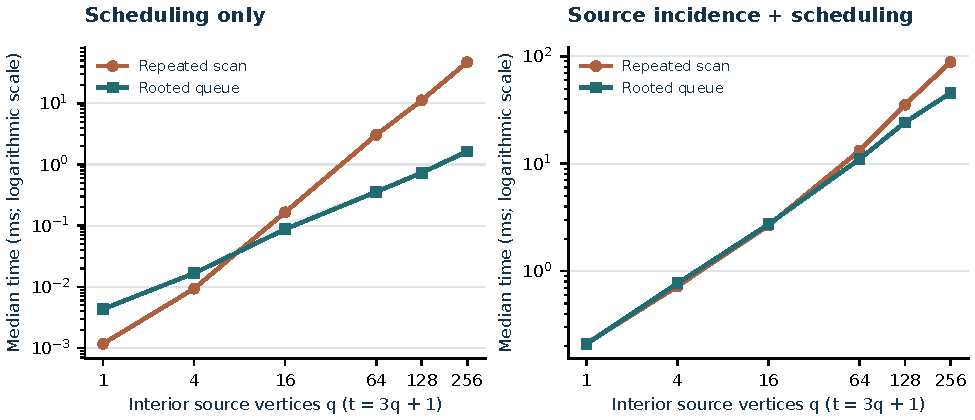
\includegraphics[width=\textwidth]{figures/local_scheduler.pdf}
\caption{Retained medians with interquartile bands. Common source work
substantially dilutes the scheduling gain. Both axes use logarithmic scales;
the two panels have different vertical ranges.}
\label{fig:timing}
\end{figure}

At $q=256$, the isolated medians are 47.098 ms for scanning and 1.636 ms
for the queue. Common source-incidence reconstruction alone takes 45.541 ms;
the directly measured combined medians are 88.425 ms and 45.655 ms. Thus
the observed ratios are $28.80$ and $1.94$, respectively. The queue has
greater constant overhead for the smallest inputs. A/A median paired ratios
range from 0.967 to 1.070; the $q=16$ ratio-of-medians A/A statistic is
noisier, 1.189. Small timing differences should not support a strong
interpretation. The largest effects are substantially larger than these
controls, but still concern a local Python implementation on a shared host.

There is also an exact asymptotic comparison independent of timing. With
$m=4q$, the old loop visits
\[
 qm-\frac{q(q-1)}2=\frac{7q^2+q}{2}
\]
rows. At $q=256$ this is 229,504 row visits and 457,462 actual interior-cap
membership tests. The queue performs 2,038 incidence updates; its explicit
upper bound including initialization is 9,426 endpoint inspections. The
old scan performs quadratic row-scan work on this genuine source family, while the new queue
has the linear structural bound of \cref{prop:cost}.

\subsection{The forest-planning experiment gives a negative result}

The native applicability audit fixes the maintained primal forest and
compares the abstract restricted planner with the ordinary rooted top queue
followed by raw core cancellation. On the 106 source cores, the restricted
planner completes 40 and refuses 66 because forced long rows already
contain a cap cycle. Ordinary core cancellation completes 100. The
restriction therefore misses 60 ordinary successes and adds no coverage.
On eight subdivided empty solid tori it completes only $q=1,2$, while
ordinary core cancellation completes all eight. This observed family is not
claimed as a theorem about every later subdivision.

These numbers concern the core before all attached bundles are resolved.
They are not the 92 whole-cut successes of \cref{tab:coverage}. In
particular, all ten former three-handle cores pass the ordinary core
consumer; the three remaining whole-cut refusals arise later.

All 114 source cores in the chain audit satisfy the uncapped
$A^{\mathsf T}B=0$ identity; 18 checks involve actual three-handles. The
mandatory set $\overline D$ is a cap forest in 40 corpus cases and two
subdivision cases. Every one has $\beta_2=0$, and the contracted rank
formula and source trace replay agree. The data do not empirically test
nontrivial forest variation: in every eligible case $|\overline D|=q$,
so the eight proposed edge orders yield the same tree. All full cores in
this audit have $\beta_2=0$. The invariance and positive-nullity statements
are supported by the proof and the explicit geometric family in
\cref{ex:geometric-cycle}, not by an overstated experimental claim.

\subsection{The exceptional-row quotient retains the missing information}

The fixed-forest quotient was checked on 21,304 ternary matrices with at
most three rows and columns, 4,096 binary $4\times3$ matrices, 3,375 legal
exceptional partitions of binary $3\times3$ matrices, and 2,000 seeded
larger matrices. Tests verify decision equivalence, exact canonical
stopping rows, lifted source schedules, ground handling, duplicate types,
and large coefficients. Separate replay verifies all 120 retained abstract
and native certificates without importing the producer.

For the ordinary fixed dual forest in the native corpus, all 106 short-row
graphs are forests. The quotient recovers the 100 complete cores and six
canonical stopping cores. In aggregate, 773 source rows reduce to 164
exceptional rows, and 809 occurring source columns reduce to 189 distinct
nonzero quotient types. The maximum exceptional-row count is nine, with
median one. All eight subdivision cores also complete. These are exact
structural compression measurements. Ordinary peeling already decides
these explicit matrices, so we claim no new measured runtime or coverage
gain from the quotient itself.

\section{Consequences for the quasipolynomial programme}
\label{sec:research}

\subsection{What the local theorem removes from the global problem}

The native source top handles need no separate combinatorial search. For
every supplied normal surface, a linear trace exists, and a single source
tree works uniformly across all its coordinate supports. A hierarchy
controller can therefore eliminate this class of three-handles before a
terminal core test without branching over possible rooted schedules merely
to obtain a valid reduction.

This does not imply that all deletion trees are interchangeable for the
later general raw problem. \Cref{sec:chain} proves interchangeability for a
specific short-row strategy, while \cref{sec:exceptional} isolates the
additional information carried by long rows. The next useful search target
is consequently the interaction of exceptional attaching curves with
forest components, rather than unrestricted enumeration of short-row
forests that homology already controls.

\begin{proposition}[Conditional preservation of a global bound]
\label{prop:global}
Suppose a correct complete hierarchy algorithm on an $n$-crossing input
visits at most $N(n)$ source states, each with encoded size at most $L(n)$.
Suppose the required source verification, top reduction, and selected
terminal operations at one state cost at most $L(n)^c$, for a fixed $c$.
Then these operations contribute at most $O(N(n)L(n)^c)$ bit work. If
both $N$ and $L$ are quasipolynomial in $n$, their contribution remains
quasipolynomial. The source top reducer adds no coordinate-support search
factor to this estimate.
\end{proposition}

\begin{proof}
Sum the stated per-state cost over the visited states. If
$N(n)\leq\exp(O((\log(n+2))^a))$ and
$L(n)\leq\exp(O((\log(n+2))^b))$, their product is
$\exp(O((\log(n+2))^{\max(a,b)}))$. The uniform source-tree theorem
supplies one valid top schedule without an enumeration of supports or trees.
\end{proof}

This is accounting, not a proof of the missing hypotheses. In particular,
polynomial verification of a supplied state does not bound the number of
candidate states, and a short hierarchy does not bound the time needed to
select its next admissible decomposing surface. The present work does not
establish either $N$ or $L$ for a complete recognizer.

\subsection{Immediate integration and performance questions}

\begin{question}[Reuse authenticated source work]
Can one immutable validated-source context serve the parallelity, boundary,
top-incidence, and terminal checks without repeating the same triangulation
and coordinate reconstruction?
\end{question}

The largest local benchmark spends more time on common incidence
reconstruction than on the new queue. This is a concrete next performance
target. A suitable design would expose source invariants through an
internally constructed object, retain exact input identity, and make
untrusted serialized objects pass the full constructor. The producer and
verifier should still have separate geometric reconstructions where
independence is part of the certificate contract. A successful change
should report whole-query timings, retained memory, and invalid-input
rejection, not only cache-hit speed.

\begin{question}[Choose a stable top policy without losing terminal cases]
When does the universal source-tree policy give the same terminal success
set as the queue, and when does a different valid top tree help with
exceptional rows?
\end{question}

The template proves validity and makes caching possible. It does not prove
optimality after the rows change. A useful experiment should compare
policies on actual source cuts, retain the full attaching records, and
separate short-row cases governed by homology from long-row cases where a
choice could matter. An abstract graph example violating the chain identity
is not suitable evidence. The minimal-subtree stopping lift provides a
specific geometric region to inspect when a policy differs.

\begin{question}[Extend the kernel to the complete finite terminal matrix]
Can the exceptional-row quotient be compiled directly on the combined
core and saturated-bundle boundary kernel, with the original geometric
projection and private-cocore accounting preserved?
\end{question}

The current quotient experiment covers cores. The seven new whole-cut
successes show that the top adapter already composes with several existing
bundle terminal paths, but the remaining obstructions occur in the full
assembly. The next adapter should retain row ownership, complete interface
circles, and the proof that omitted private columns cannot become valid
pivots. It should then lift a quotient stopping set to the corresponding
source annuli and core attaching curves. This would produce a better
description of each unresolved whole cut, without claiming that the
description itself resolves it.

\subsection{Geometric questions that could change the asymptotics}

\begin{question}[Transport a full inherited boundary pattern]
Can the two/three-handle collar homeomorphisms be encoded and composed in
polynomial bit size while transporting arbitrary admissible pattern curves
and trivalent graphs?
\end{question}

For the current parallelity ports, support avoidance makes the relative map
simple. A general pattern may cross the support. One possible approach is
to retain local PL boundary maps as a composition grammar, with source
flags and affine rank intervals on each patch. The hard part is then an
exact intersection and admissibility checker that operates on the grammar
without expanding its maps. The needed theorem must bound both the grammar
and the complexity of the queries used by the next hierarchy step. A
short list of moves alone does not bound the expanded boundary pattern.

\begin{question}[Exploit few exceptional rows]
For a geometrically authenticated state with $k$ exceptional rows, can a
complete useful family of forest changes or local geometric repairs be
searched in $(t+b_x)^{O(k+1)}$ time, or with another bound that becomes
quasipolynomial when $k$ is logarithmic?
\end{question}

This is a proposed target, not a conjecture supported by a proof. The
fixed-forest quotient gives an exact state description and at most
$3^k-1$ nonzero capped column types. It does not show that the set of all
such descriptions reachable by forest changes is small, nor that local
changes preserve completeness of a search. A serious attempt should first
seek a counterexample to any claimed exchange axiom or locality bound.
\Cref{prop:not-matroid} already rules out the simplest unrestricted
matroid formulation.

\begin{question}[Change the primal forest and cocore system]
Can a primal zero/one-handle forest be chosen so that the number or total
interaction complexity of the exceptional rows is provably small?
\end{question}

The homological rigidity theorem fixes that forest. Changing it changes the
surviving columns and can change which attaching curves are short. This
is a more plausible source of useful freedom than short-row dual-tree
exchange. The exact parameter to minimize should incorporate geometry:
the number of long rows alone ignores the number and placement of their
pin columns in the quotient. A proposed optimization should retain a
certificate for the cocore correspondence and should not substitute free
group exponent reduction for geometric intersection reduction.

\begin{question}[Destroy a lifted stopping core by controlled geometric moves]
Which handle slides, disk exchanges, or boundary bigon removals can reduce
the unsigned intersection data near a lifted stopping set while preserving
the marked manifold and a useful global complexity measure?
\end{question}

The exact lift identifies the exceptional rows and the short-tree paths
that keep them blocked. It therefore localizes a candidate repair region.
It does not prove that a necessary repair is confined there. The desired
statement would give a complete family of repairs, a compact proof for
each move, and a potential that decreases by a controlled amount. A
counterexample where all useful repairs leave this region would be equally
valuable, because it would rule out an attractive but incomplete search.

\begin{question}[Batch compressed primitive reductions]
Can large families of equivalent curve slides be accelerated in the
compressed source coordinates, with an exact geometric certificate for
their combined effect?
\end{question}

Compressed free-group primitivity is a relevant comparison, but it is not a
replacement for embedded curve data. Kapovich's 2026 work distinguishes
rank-two polynomial algorithms from more general compressed settings and
gives the family $ab^{2^n}$ as a warning about exponentially many elementary
Whitehead descent steps~\cite{kapovich2026}. A geometrically useful batching
theorem must specify how an accelerated algebraic step acts on the actual
boundary curves, their disjointness, and the protected pattern. Large binary
coordinates make batched operations attractive precisely because expanding
the implied elementary moves defeats the objective.

\subsection{Global control and verification questions}

\begin{question}[Find a stable hierarchy potential]
Is there a potential on authenticated marked source states whose decrease
controls both useful-surface selection and the cost of rebuilding the
compressed representation?
\end{question}

Removing top handles changes two handle counts equally and preserves Euler
characteristic. It is not by itself a strict decrease of a global
topological complexity. The potential must account for source size,
coordinate bit length, pattern complexity, and any reset that invalidates
cached geometry. A bound on the number of moves inside a phase is
insufficient if the next phase rebuilds a much larger state. A candidate
proof should state a recurrence for these quantities together, rather than
prove separate bounds that depend circularly on one another.

\begin{question}[Control useful surface discovery]
Can the existing separator, first-return, and surface-batch proposals be
connected to an authenticated complete choice of the next decomposing
surface, with explicit bit bounds?
\end{question}

The incoming reports provide several useful compressed graph and normal
coordinate operators. Their output graphs, surfaces, and retained marks
must still be connected to the admissibility and essentiality conditions
of a complete hierarchy. The source top theorem can be used after such a
choice; it does not make the choice complete. A deliverable at this stage
should include both a source exporter and a negative certificate describing
what exhaustive failure means in the chosen restricted problem.

\begin{question}[Make the source interface reentrant]
Can later hierarchy states with several boundary components be accepted
by a generalized source constructor without losing the topology and
pattern checks now guaranteed at the one-torus entry point?
\end{question}

The relative top theorem already permits several nonempty boundary
components. The native validator does not. Generalizing it is more than
removing the torus test: all consumers of boundary component counts,
compressing disks, source provenance, and essential-pattern criteria must
be given explicit contracts. This is a natural point to connect the
initial knot-diagram provenance certificate to the sequence of derived
states.

\begin{question}[Mechanize the small certificate kernel]
Which of the cap inventory, rooted trace, graphic peeling, and quotient
stopping-lift lemmas can be formalized first, while keeping the required
PL geometric theorem explicit?
\end{question}

The finite combinatorial checker is small enough to make formalization
realistic. A useful first milestone is a theorem that every accepted trace
has the exact graph and row consequences stated here. The source geometry
then remains a clearly named theorem connecting that finite kernel to
embedded handles. Python tests and independent implementations provide
strong regression evidence but are not machine-checked proofs of the PL
statement.

The highest-value next steps are the source-context optimization, the full
terminal stopping lift, and a marked geometric repair operation with a
proved completeness or progress property. They address observed costs or
specific unresolved geometry. Another abstract forest optimizer without
the chain and embedding constraints would not address the main barrier
identified by this work.

\appendix
\section{Reproduction and artifact map}
\label{sec:reproduction}

\subsection{Pin the input before applying the change}

The integration patch is relative to the ProveIt repository root. Its target
commit is\par\noindent\sourcecommit.\par
Its manifest records the SHA-256 of every supplied
file and the original hash of each modified file. The package does not
include or apply any of the ten incoming ZIP patches.

For a clean comparison, retain one checkout at that commit and apply
\smallpath{integration/proveit-relative-top-handles.patch} to another.
The command \code{git apply --check} should succeed before applying it.
The parallel \smallpath{integration/overlay/} tree is a convenient full-file
alternative. It is not an additional patch to apply afterwards.

\subsection{Run the focused release checks}

Set \code{PACK} to the absolute unpacked package path and \code{FAST} to
the target repository's \smallpath{Topology/UnknotRecognition/fast} path.
Then run:
\begin{quote}\small
\begin{verbatim}
python "$PACK/tools/run_targeted_tests.py" \
  --fast-dir "$FAST" --output-dir /tmp/top-release-check

cd "$FAST"
python core_top_research/audit.py \
  --fast-dir "$FAST" \
  --reference ../synthesis/data/boundary-kernel-audit.json \
  --oracle-top --output /tmp/extended-audit.json \
  --save-certificates /tmp/new-top-certificates
\end{verbatim}
\end{quote}
The test runner selects the eight named focused modules and writes a full
log plus machine-readable counts. All 67 methods pass in the separate clean
patch application. The runner also requires the unchanged source fixtures
\smallpath{synthesis/data/core-three-handle-probe.json},
\smallpath{synthesis/data/handle-reducible-trefoil.json}, and
\smallpath{reports/57/results/discovery_corpus.json}, relative to
\smallpath{Topology/UnknotRecognition/}; it checks these before starting.
The corpus audit requires the retained
reference JSON and compares all 106 cases; \code{--oracle-top} uses Regina
for fresh explicit cuts on the ten former exclusions. Omit that flag when
only the native source replay is required. These fresh explicit checks can
be more expensive than the compressed native operation.

The current audit script can also test a baseline checkout by pointing
\code{--fast-dir} at its unmodified fast directory and omitting
\code{--oracle-top}. The script itself must be invoked from the new package
or overlay, since it is not part of the pinned baseline.

\subsection{Reproduce local and structural experiments}

From the patched fast directory:
\begin{quote}\small
\begin{verbatim}
python core_top_research/benchmark.py \
  --output /tmp/top-scheduler-benchmark.json
python core_top_research/template_audit.py \
  --output /tmp/template-audit.json
python core_top_research/forest_audit.py \
  --output /tmp/forest-exchange-audit.json
python core_top_research/chain_audit.py \
  --subdivision-source /tmp/forest-exchange-audit.json \
  --output /tmp/chain-compatibility-audit.json
cp /tmp/forest-exchange-audit.json \
  core_top_research/forest_exchange_audit.json
python core_top_research/residual_kernel_audit.py \
  --output /tmp/residual-kernel-audit.json
python core_top_research/residual_kernel_audit.py \
  --replay-only "$PACK/evidence/residual_kernel_audit.json"
\end{verbatim}
\end{quote}
The default benchmark uses the reported six sizes, nine scheduler/A--A
pairs and five combined-stage pairs. Hardware and load changes can alter
timings; the exact work counts, source hashes, and proof consequences are
the reproducible mathematical comparisons. The residual-kernel audit
recreates its finite matrix tests and the native corpus. Its subdivision
fixtures are read from the required neighbouring file
\smallpath{core_top_research/forest_exchange_audit.json}; the copy command
above supplies that file. Alternatively, copy the archive's retained
\smallpath{evidence/forest_exchange_audit.json} to that location before the
kernel audit. The replay-only command reads its supplied JSON directly.

\subsection{Build the article and inspect the evidence}

All TeX sections and the vector timing figure are included. From
\smallpath{article/}, build with
\begin{quote}\small
\begin{verbatim}
latexmk -pdf -interaction=nonstopmode -halt-on-error \
  Relative_Top_Handles.tex
\end{verbatim}
\end{quote}
The article uses standard TeX Live packages. The optional
\smallpath{tools/render_evidence.py} regenerates the timing table and figure
from the retained JSON with Matplotlib. It does not run a new measurement.

The key evidence files are:
\begin{center}\small
\begin{tabular}{@{}p{0.42\textwidth}p{0.53\textwidth}@{}}
\toprule
File under \path{evidence/} & Contents\\
\midrule
\path{baseline_audit.json}, \path{extended_audit.json}
& Per-case results, source corpus hash, proof sizes, and oracle comparisons\\
\path{new_certificates/}
& Exact source/vector inputs and all seven new whole-cut certificates\\
\path{top_scheduler_benchmark.json}
& Six real source triangulations, both traces, operation counts, raw paired
samples, A/A controls, and stage timings\\
\path{template_audit.json}
& Fixed source tree, 64 compatible vectors, and binary-scale proofs\\
\path{forest_exchange_evidence.json}
& Abstract planner examples, independent replays, and exhaustive-test summary\\
\path{forest_exchange_audit.json}
& Native restricted-strategy results and eight subdivision fixtures\\
\path{chain_compatibility_audit.json}
& Uncapped source matrices, chain checks, ranks, mandatory cycles, and traces\\
\path{residual_kernel_audit.json}
& Quotient matrices, source lifts, exact stopping rows, and retained replay cases\\
\bottomrule
\end{tabular}
\end{center}

\subsection{Claim boundaries for later integration}

The article gives mathematical proofs, and the package gives independent
programmatic replay and regression evidence. It is not a formal proof
assistant development. The abstract failure witnesses establish a failure
of a named matrix strategy. The native whole-cut successes establish
unmarked handlebody censuses for specified cuts. Neither is automatically
a final essential-boundary-pattern certificate or an unknot verdict.

The archive's claim ledger and integration notes repeat these contracts so
that a future importer need not infer them from benchmark filenames. All
third-party sources are referenced by public links; their full papers or
lecture slides are not redistributed in this package.

\section{Repository and incoming-work audit}
\label{sec:source-audit}

The review used the maintained source at the pinned commit and the ten ZIP
files then present under \smallpath{docs/incoming}. The incoming audit
covered READMEs, abstracts, relevant theorem statements and proofs,
implementation boundaries, and research agendas. It is a targeted overlap
audit, not a claim that every proof in every imported manuscript was
independently verified. File hashes and the more detailed audit notes are
included with the deliverables.

\begin{longtable}{@{}p{0.25\textwidth}p{0.69\textwidth}@{}}
\toprule
Incoming topic & Relevant existing result and boundary of overlap\\
\midrule
\endfirsthead
\toprule
Incoming topic & Relevant existing result and boundary of overlap\\
\midrule
\endhead
\bottomrule
\endfoot
Cographic Persistence
& Surface-batch independence, cographic optimization, and rebuild accounting.
Its matroid concerns retaining decomposing surfaces, not selecting source
two/three-handle deletion trees.\\[4pt]
Disconnected Tile Kernels
& Compressed graph operators for disconnected repeated tiles, with contextual
replacement. It does not authenticate source top-handle geometry.\\[4pt]
Genus Budgets and Native Interfaces
& Initial source handle compilation and reduction, genus budgets, and native
interface data. The initial two/three queue is credited; the later normal-cut
adapter with preserved ports is the extension here.\\[4pt]
Modular Morse Certificates
& Verification of supplied interval matchings and relative product lifts.
No general matching discovery or native exceptional-three-handle adapter is
supplied.\\[4pt]
Moment-Coded First Returns
& Weighted orbit summaries, transport, and first-return compression. These
are source data operators, not the relative top-handle move proved here.\\[4pt]
Saturated Bundle Cancellation
& Geometric residual relations for saturated bundles, private-cocore
projection, and 85/106 native censuses. The unsupported three-handles are an
explicit remaining problem.\\[4pt]
Scalar Separators
& Exact restricted normal-coordinate message rules and a separator
obstruction. This concerns surface discovery, not top-handle elimination.\\[4pt]
Unknot Hierarchy Kernels
& Relative bands for nonsaturated bundles, bounded core kernels, and
repeated-component graph reductions. Saturated relations and three-handles
remain distinct obligations.\\[4pt]
Sparse Cut Grammars
& Exact compressed graph cut responses and contextual interfaces. A faithful
geometric source exporter and embedded noose transport remain necessary.\\[4pt]
Stopping Cores
& Complete unit-column characterization of positive raw cancellation,
canonical stopping sets, passenger transport, and native saturated tests.
Its completeness theorem is reused; the cap-forest chain constraint and
exceptional short-tree quotient are new relative to this inspected work.\\
\end{longtable}

The maintained \smallpath{synthesis/data/core-three-handle-probe.py} already
computes candidate cap endpoints, removes rooted pairs, and predicts seven
successful downstream cases. Its own stated limitation is missing
independent source replay. We therefore do not present the diagnostic's
initial idea or its seven predictions as newly discovered. The advance is
the relative proof, orientation-safe reconstruction, uniform source
template, strict compositional certificate, and demonstrated integration.

The source core bounds and rank charts come from the maintained
\smallpath{normal_parallelity_geometry.py} and its independent
\smallpath{normal_parallelity_reference.py}. The geometric occurrence
matrix is read from complete attaching-cycle flags. The prior initial
source queue in \smallpath{source_handle_reduction.py} confirms that
boundary-rooted cancellation is already part of the project's vocabulary;
it did not by itself justify the new relative normal-cut use.

Novelty is consequently claimed at the level supported by this audit:
specific source-relative theorems and adapters, the chain-aware analysis of
the proposed forest optimization, and the exact exceptional-row stopping
quotient. Classical handle cancellation, graphic matroids, matroid
partition, and stopping-set theory are acknowledged as underlying tools.
No assertion is made that the full literature contains no equivalent
formulation of any elementary graph lemma.

\begin{thebibliography}{99}
\addcontentsline{toc}{section}{References}

\bibitem{lackenby2026}
Marc Lackenby,
\emph{Incompressible surfaces, hierarchies and unknot recognition},
arXiv:2607.23350v1, 25 July 2026.
In particular Sections~9--10 and Theorem~14.1.
\url{https://arxiv.org/abs/2607.23350v1}.

\bibitem{oxford2021}
Marc Lackenby,
\emph{Unknot recognition in quasi-polynomial time},
February 2021 lecture slides, 109 pages; announcement on PDF pp.~13--14.
\url{https://people.maths.ox.ac.uk/lackenby/quasipolynomial-talk.pdf}.
The later Oxford slide version is distinct; the cited bound here is from
this February version. Slides are referenced, not redistributed.

\bibitem{jackson2023}
Adele Jackson,
\emph{Minimal triangulation size of Seifert fibered spaces with boundary},
arXiv:2301.02085v1, 5 January 2023.
Lemma~3.2 and the following parallelity discussion, pp.~6--7.
\url{https://arxiv.org/abs/2301.02085v1}.

\bibitem{edmondsfulkerson}
Jack Edmonds and D.~R.~Fulkerson,
\emph{Transversals and matroid partition},
Journal of Research of the National Bureau of Standards, Section B,
69B(3) (1965), 147--153.
Theorem~1c, constructive exchange proof, and contraction formula.
\url{https://doi.org/10.6028/jres.069B.016}.
Original publication:
\url{https://nvlpubs.nist.gov/nistpubs/jres/69B/jresv69Bn3p147_A1b.pdf}.

\bibitem{kapovich2026}
Ilya Kapovich,
\emph{Compressed primitivity problem in free groups},
arXiv:2607.21499v1, July 2026.
Theorems~1.1--1.2 and Example~1.3.
\url{https://arxiv.org/abs/2607.21499v1}.

\bibitem{repo}
Vladimir Reshetnikov and ProveIt contributors,
\emph{ProveIt: Topology/UnknotRecognition},
repository snapshot \sourcecommit, inspected 12 October 2026.
The maintained source, synthesis reports, retained corpus, and diagnostic
script are identified in the text and package manifest.
\url{https://github.com/VladimirReshetnikov/ProveIt/tree/8cb7d9d25ac8cb64a9d147304e3441e98e94c7a4/Topology/UnknotRecognition}.

\bibitem{incoming-stopping}
ProveIt incoming research package,
\emph{Stopping Cores}, 12 October 2026.
\smallpath{docs/incoming/ProveIt_Unknot_Stopping_Cores_2026-10-12.zip}
at the snapshot in~\cite{repo}. Used for stopping-set persistence,
completeness of positive raw cancellation, and geometric projection scope.

\bibitem{incoming-saturated}
ProveIt incoming research package,
\emph{Saturated Bundle Cancellation}, 12 October 2026.
\smallpath{docs/incoming/ProveIt_Saturated_Bundle_Cancellation_2026-10-12.zip}
at the snapshot in~\cite{repo}. Used for source annulus charts, residual
bundle relations, private-cocore projection, and overlap analysis.

\bibitem{incoming-genus}
ProveIt incoming research package,
\emph{Genus Budgets and Native Interfaces}, 12 October 2026.
\smallpath{docs/incoming/ProveIt_Genus_Budgets_Native_Interfaces_2026-10-12.zip}
at the snapshot in~\cite{repo}. Used for initial source reduction and
interface compilation context.

\bibitem{incoming-collection}
ProveIt incoming research collection, 12 October 2026.
The ten package titles and exact overlap boundaries are listed in
\cref{sec:source-audit}; their hashes are retained in the package audit.
\url{https://github.com/VladimirReshetnikov/ProveIt/tree/8cb7d9d25ac8cb64a9d147304e3441e98e94c7a4/docs/incoming}.

\end{thebibliography}

\end{document}
